%!TEX root = ../dissertation.tex
\chapter{RF cryostats}
\label{appen:RF_cryostats}
\newthought{All experiments reported} in this thesis were performed in one of three cryostats, each wired for high frequency measurements. A custom sample mounting board was machined from copper laminated PTFE (Rogers Corp, RT/duroid\textsuperscript{\textregistered}), as shown in Fig.~\ref{Fig:Appen:sample_board}. Five coplanar waveguides, with characteristic impedance $50~\Omega$, are milled into the circuit board along with 14 DC lines and a DC ground. Each RF waveguide ends in a through board SMP male connector while all DC lines and the DC ground connect to a through board ``NanoD" connector. The entire circular board measures $1$ inch in diameter allowing it to lowered into the small bore of a superconducting magnet. 

The sample and SMD inductors/capacitors are fixed to the board using double sided Kapton tape and all componets are wired together using either solder or direct wirebonding. Fig.~\ref{Fig:Appen:sample_LC} shows an example of a double stage match network connected using only wirebonds. In practice, aluminum wire bonds have difficulty bonding to the soft connectors of the SMD capacitors and so often solder is used for these parts. Once connected, the sample is sealed in an RF tight copper box which can loading into any of the three cryostats described below.

\begin{figure}
\centering
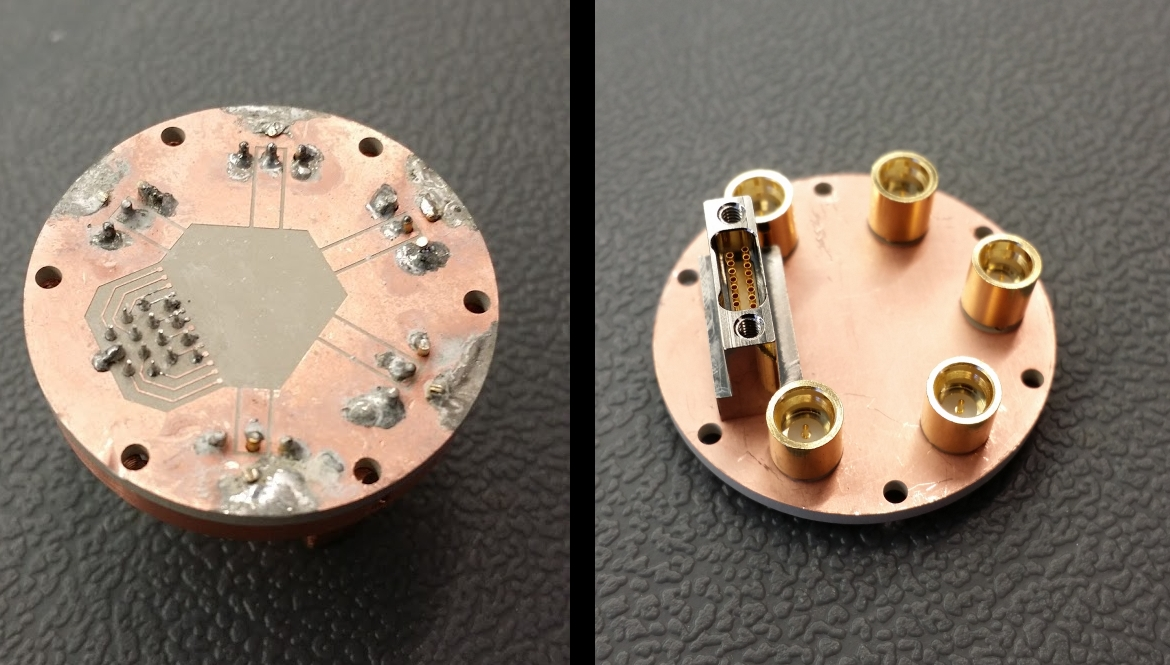
\includegraphics[width=0.8\textwidth]{figures/appendix/cryostats/sample_package.jpg}
\caption{Images of the circuit board used to mount samples. (\textbf{Left}) sample is placed in the copper free area in the center of the board. Five coplanar waveguides are milled along the outer ring. 14 DC lines with bonding pads and a DC ground are machined on one end. (\textbf{Right}) the backside of the circuit board where each RF waveguide is soldered to an SMP connector and all DC lines are soldered to the pins on a ``NanoD" connector.}
\label{Fig:Appen:sample_board}
\end{figure}

\begin{figure}
\centering
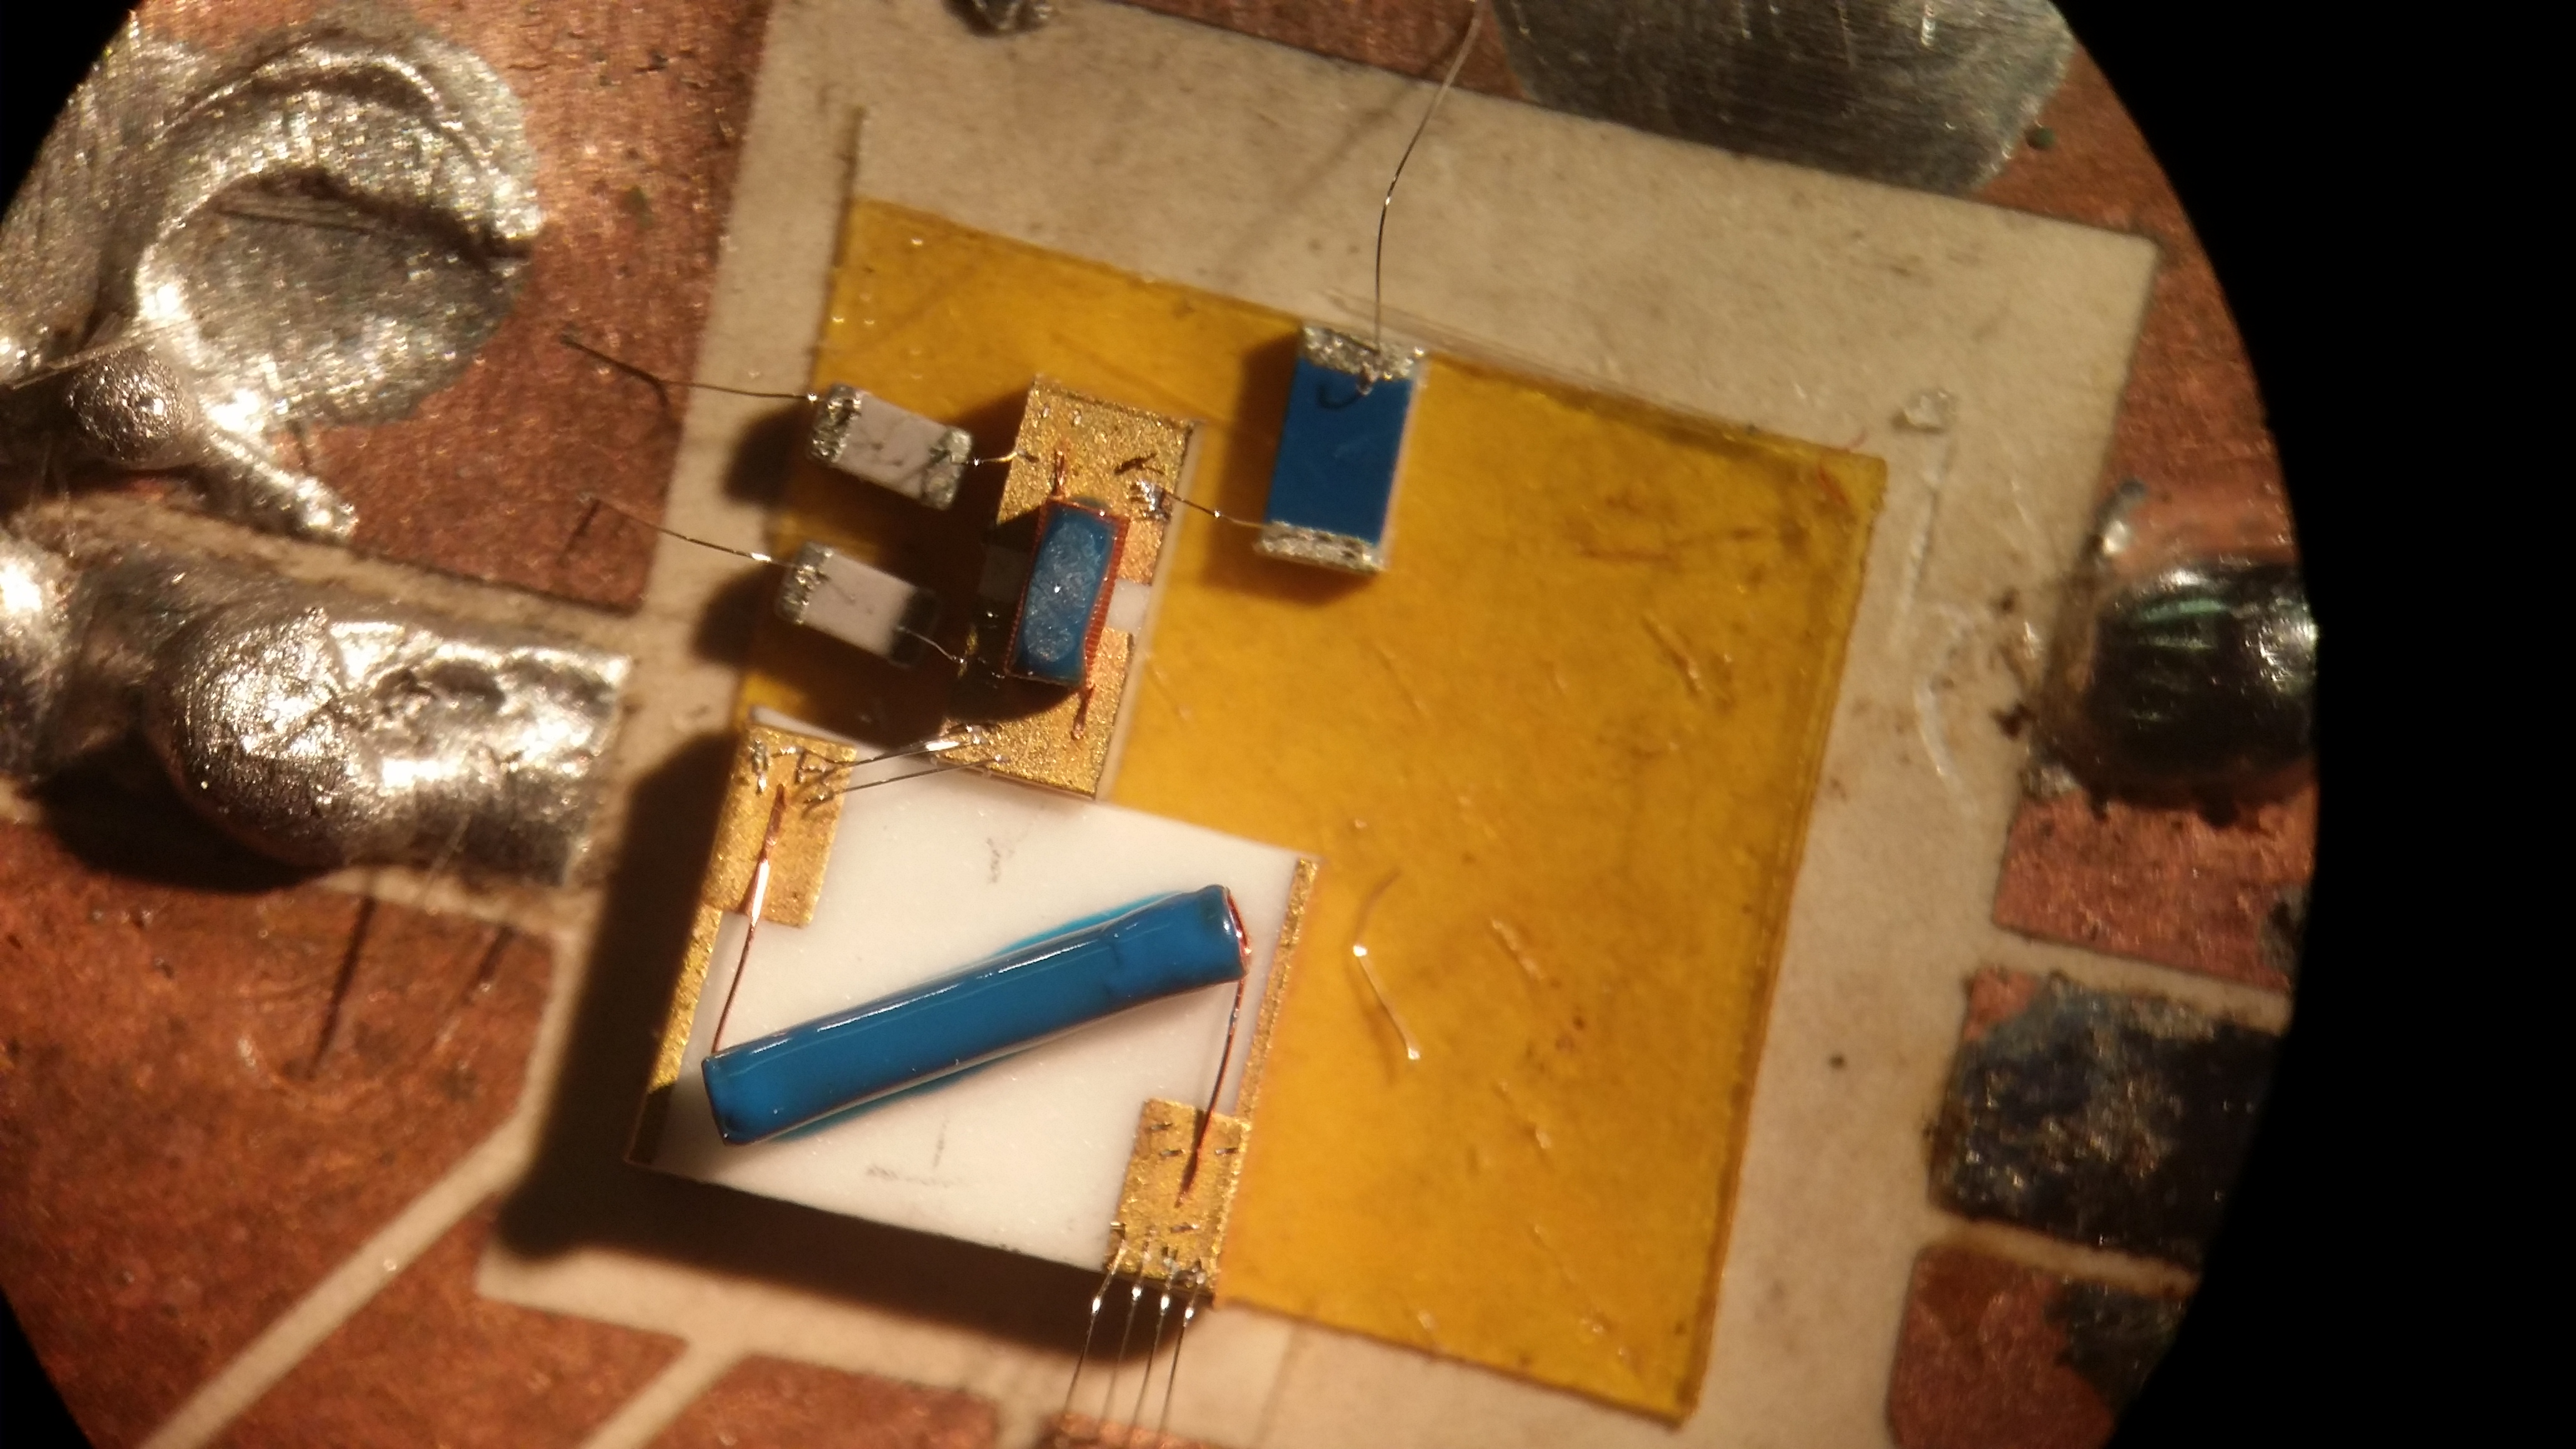
\includegraphics[width = 0.8\textwidth]{figures/appendix/cryostats/sample_LC.jpg}
\caption{Example of components mounted on our circuit board. In this case, 2 inductors (blue elements with gold leads), 2 capacitors (grey elements with silver leads), and one resistor (blue element with silver leads) forming a two-stage LC matching network. Components are secured using double-sided Kapton tape and connected using aluminum wirebonds.}
\label{Fig:Appen:sample_LC}
\end{figure}


\section{Janis}

\newthought{The experiments discussed in chapters \ref{ch:thermal_conductance_in_high_density_graphene} and \ref{ch:the_Dirac_fluid}} were performed in one of two $^4$He closed cycle Janis SHI-4 cryocoolers located at Raytheon BBN Technologies and Harvard University. The Harvard system is shown in Fig \ref{Fig:Appen:Janis} and operates with the sample in vacuum over a continuous temperature range of $2.8-320~K$. Custom copper thermalization plates were machined to thermally anchor SMA bulkheads at $50~K$ and base temperature. Solid, semi-rigid coaxial cables with copper inner and outer conductors are run through the system. Often cryogenic filters are placed at the $50~K$ stage to help reflect high frequency thermal noise from room temperature. A heater and thermometer are mounted on the sample stage to control and measure the bath temperature using a Lakeshore PID controller. The sample package described above is mounted on a pedestal and bolted directly onto the base plate. For experiments that do not require ultra-low temperatures or magnetic fields, this system is my personal favorite as its versatile, reliable, and easy to maintain.
\begin{figure}
\centering
\includegraphics[width = 0.8\textwidth]{figures/appendix/cryostats/Janis.jpg}
\caption{Janis SHI-4 cryocoolor used in parts of this dissertation. (\textbf{Left}) image of the closed system sealed and under vacuum. Optical windows are available but are blocked for these experiments. (\textbf{Right}) image of the opened system exposing the RF semi-rigid coax cables. The sample package is mounted onto the top plate which is cooled via a closed cycle $^4$He system and the temperature is set using a heater, thermometer, and Lakeshore PID controller. Low-pass filters are placed at the mid temperature plate to reflect room temperature noise.}
\label{Fig:Appen:Janis}
\end{figure}

\section{Oxford}
\label{Appen:Oxford}
\newthought{The Oxford brand cryostat}, used for the bulk of chapter \ref{ch:magneto-thermal_transport}, is a wet $^4$He system with a variable temperature insert (VTI) capable of operating from $1.7-300~K$. It houses a $14~T$ superconducting magnet with a relatively small ${\sim}1.1$  inch bore. The sample is inserted into the VTI and cooled via cold $^4$He vapor which is held at a fixed temperature by a heater and thermometer located at the vapor inlet and controlled by a Lakeshore PID controller. 

\begin{figure}
\centering
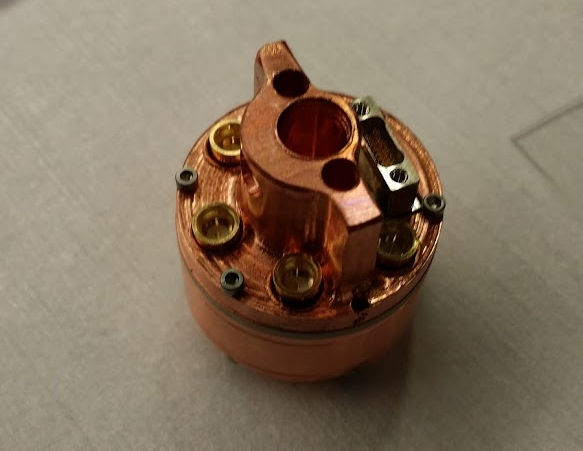
\includegraphics[width = 0.5\textwidth]{figures/appendix/cryostats/Oxford_package.jpg}
\caption{Sample package mounted to the custom adapter made for the Oxford cryostat. Adapter has two machined holes to house a heater and thermometer. Entire package is then affixed to the end of a long SS thin-walled tube and lowed into the Oxford VTI.}
\label{Fig:Appen:Oxford_package}
\end{figure}

The sample package described above is attached via non-magnetic SS screws to a custom copper adapter, as shown in Fig. \ref{Fig:Appen:Oxford_package}. This custom adapter is was machined to house a Cernox\textsuperscript{\textregistered} thermometer (Lakeshore AA package) and resistive cartridge heater. The entire package can then be affixed onto the end of a long SS thin-walled tube and held in place by a set screw, as shown in Fig. \ref{Fig:Appen:Oxford_Probe}. A copper plate in affixed to the tube about $1$ foot above the sample package and contains space for up to 6 SMA bulk head connectors. Five semi-rigid coax are run from room temperature SMA bulkhead feedthroughs to this mid temperature copper plate; two of these coax have copper inner and outer conductors and are used for noise measurements while the rest are an alloy of Copper and Nickel (to reduce the thermal conductance to the sample) and are used as excitation lines and/or gate control lines. Low-pass filters are often placed on the mid-temperature plate to reflect high frequency noise from room temperature. The heater and thermometer lines are connected to a DC military feedthrough and the nanoD is connected to a Fisher feedthrough.

\begin{figure}
\centering
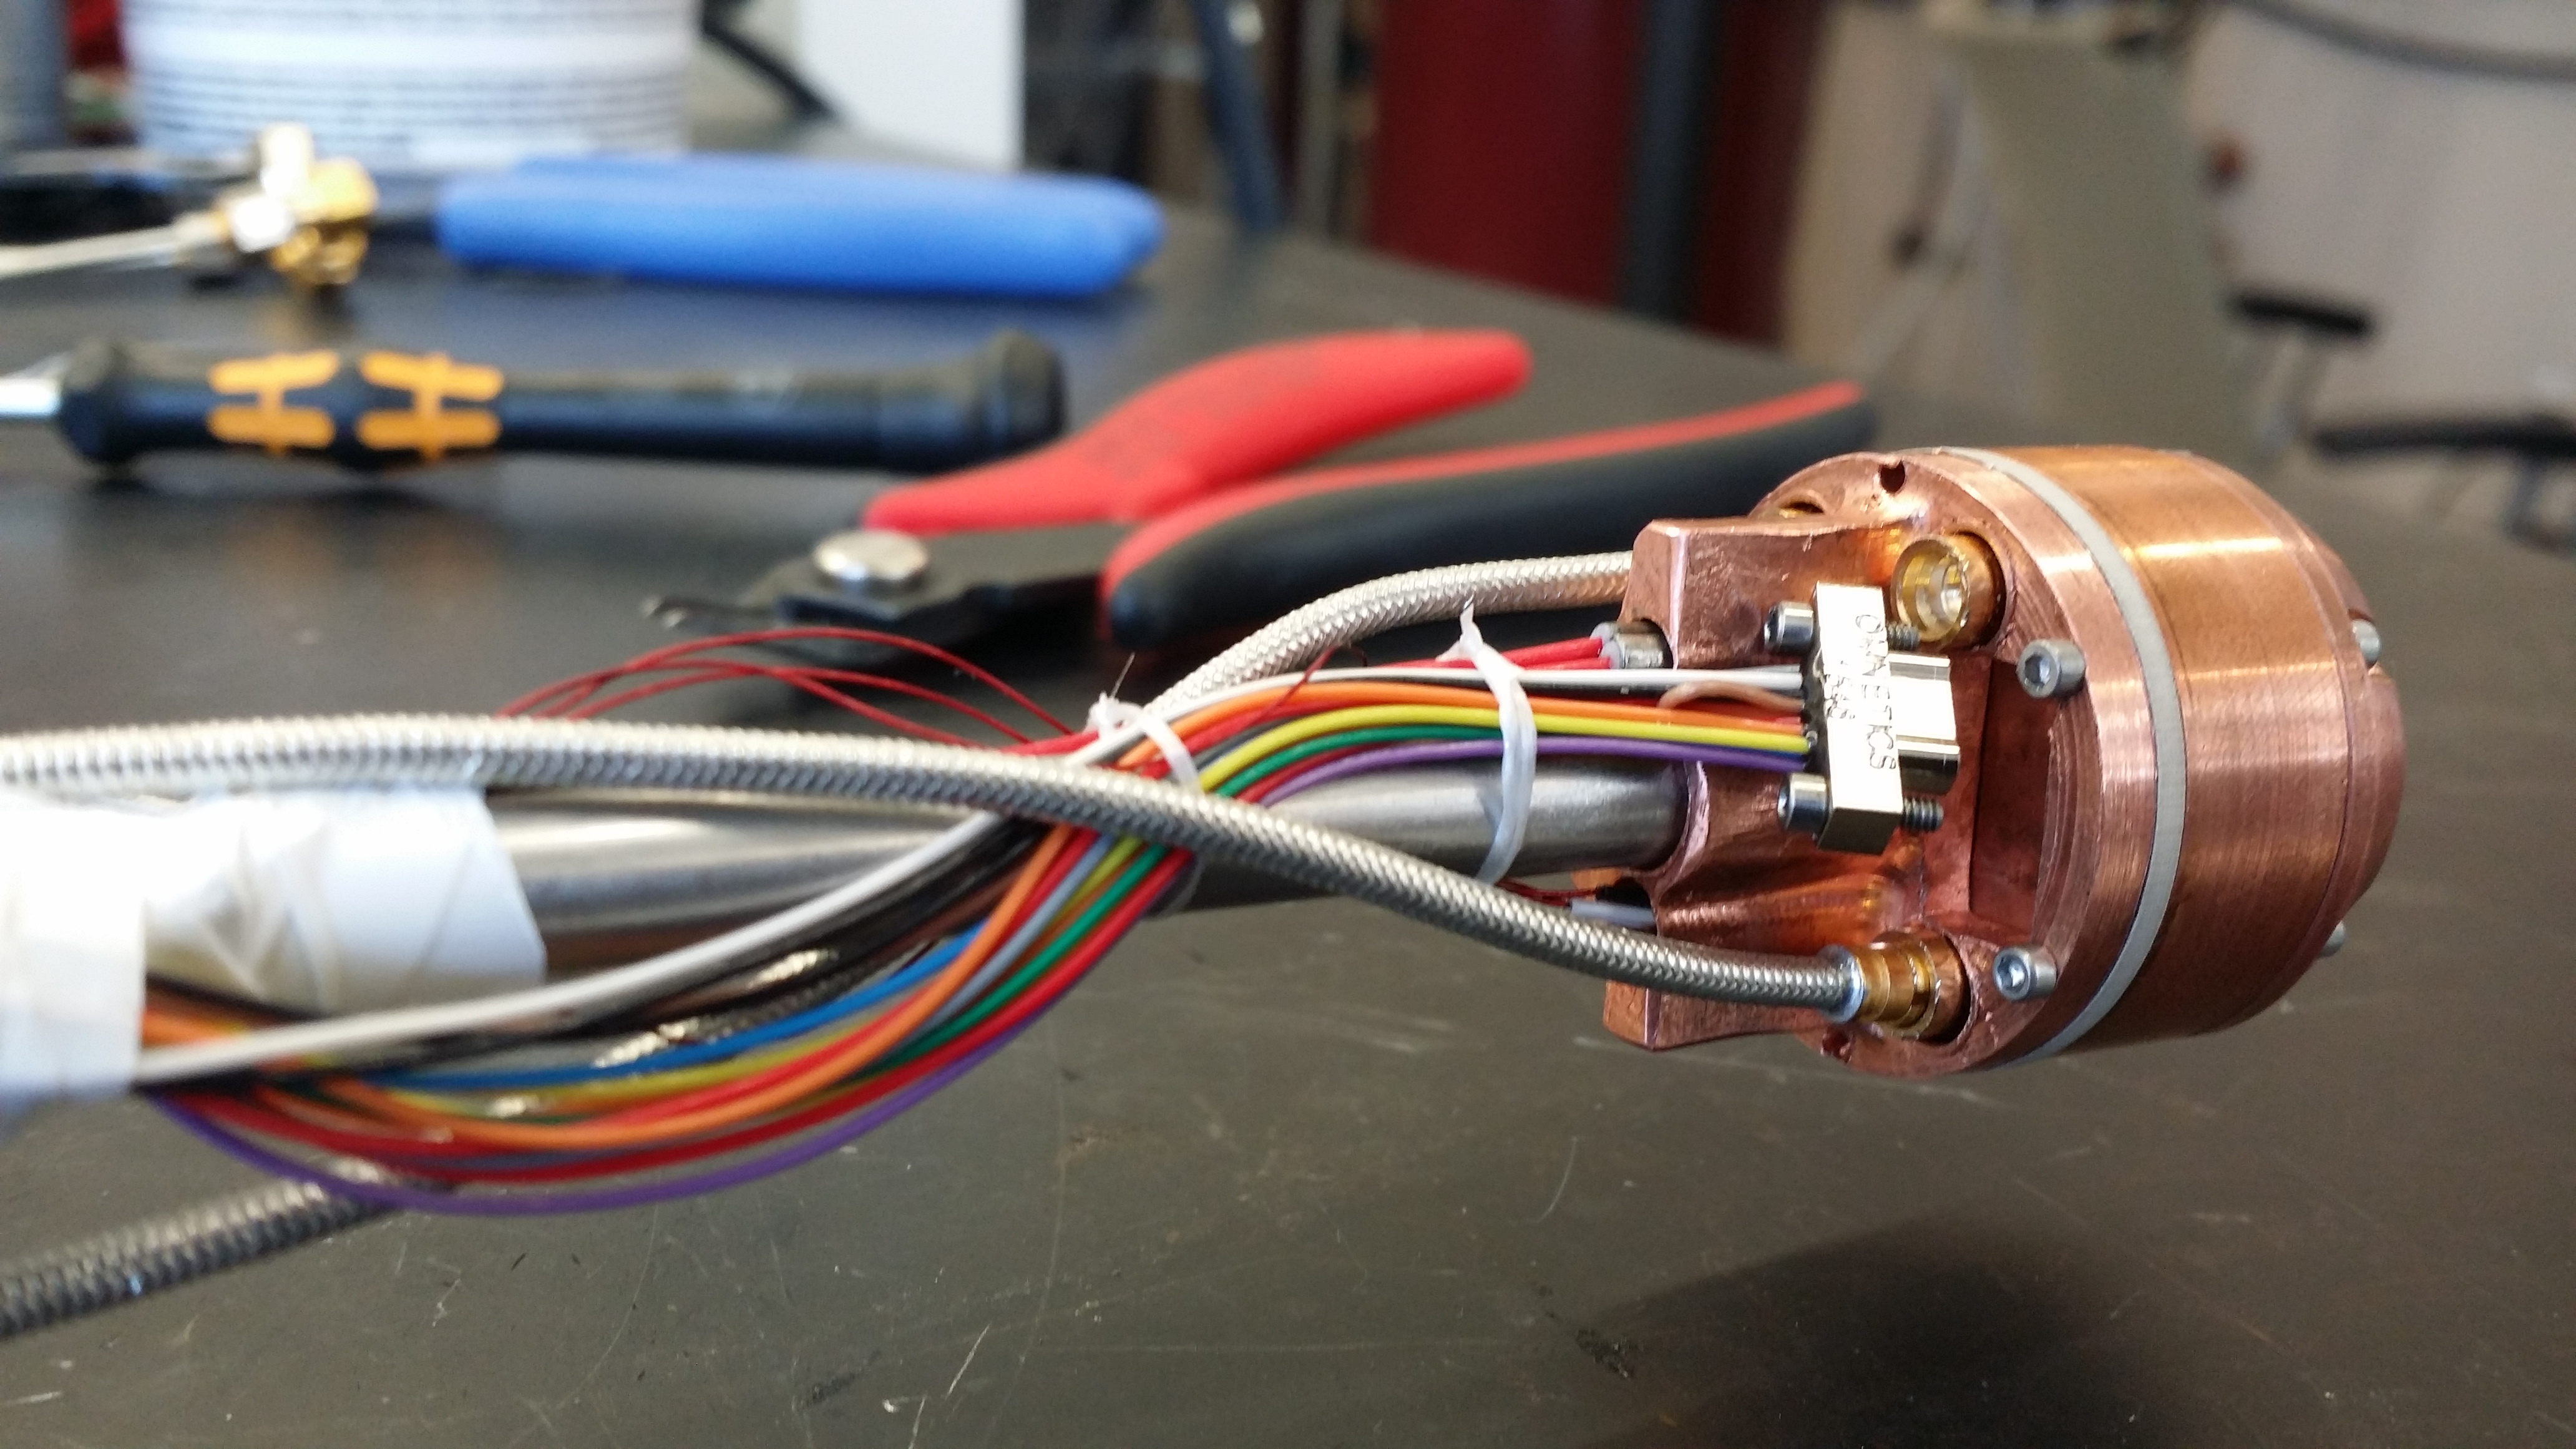
\includegraphics[width = 0.8\textwidth]{figures/appendix/cryostats/Oxford_probe2.jpg}
\caption{The business end of the custom made RF measurement probe for the Oxford VTI. The sample package is affixed to a SS tube using a set screw. RF coaxial measurement lines connect the on-board SMP connectors to the room temperature SMA bulkhead feedthroughs. DC connections are made via a nanoD connector (the nanoD plug is removed in this image as DC lines were not needed in this experiment).}
\label{Fig:Appen:Oxford_Probe}
\end{figure}

\begin{figure}
\centering
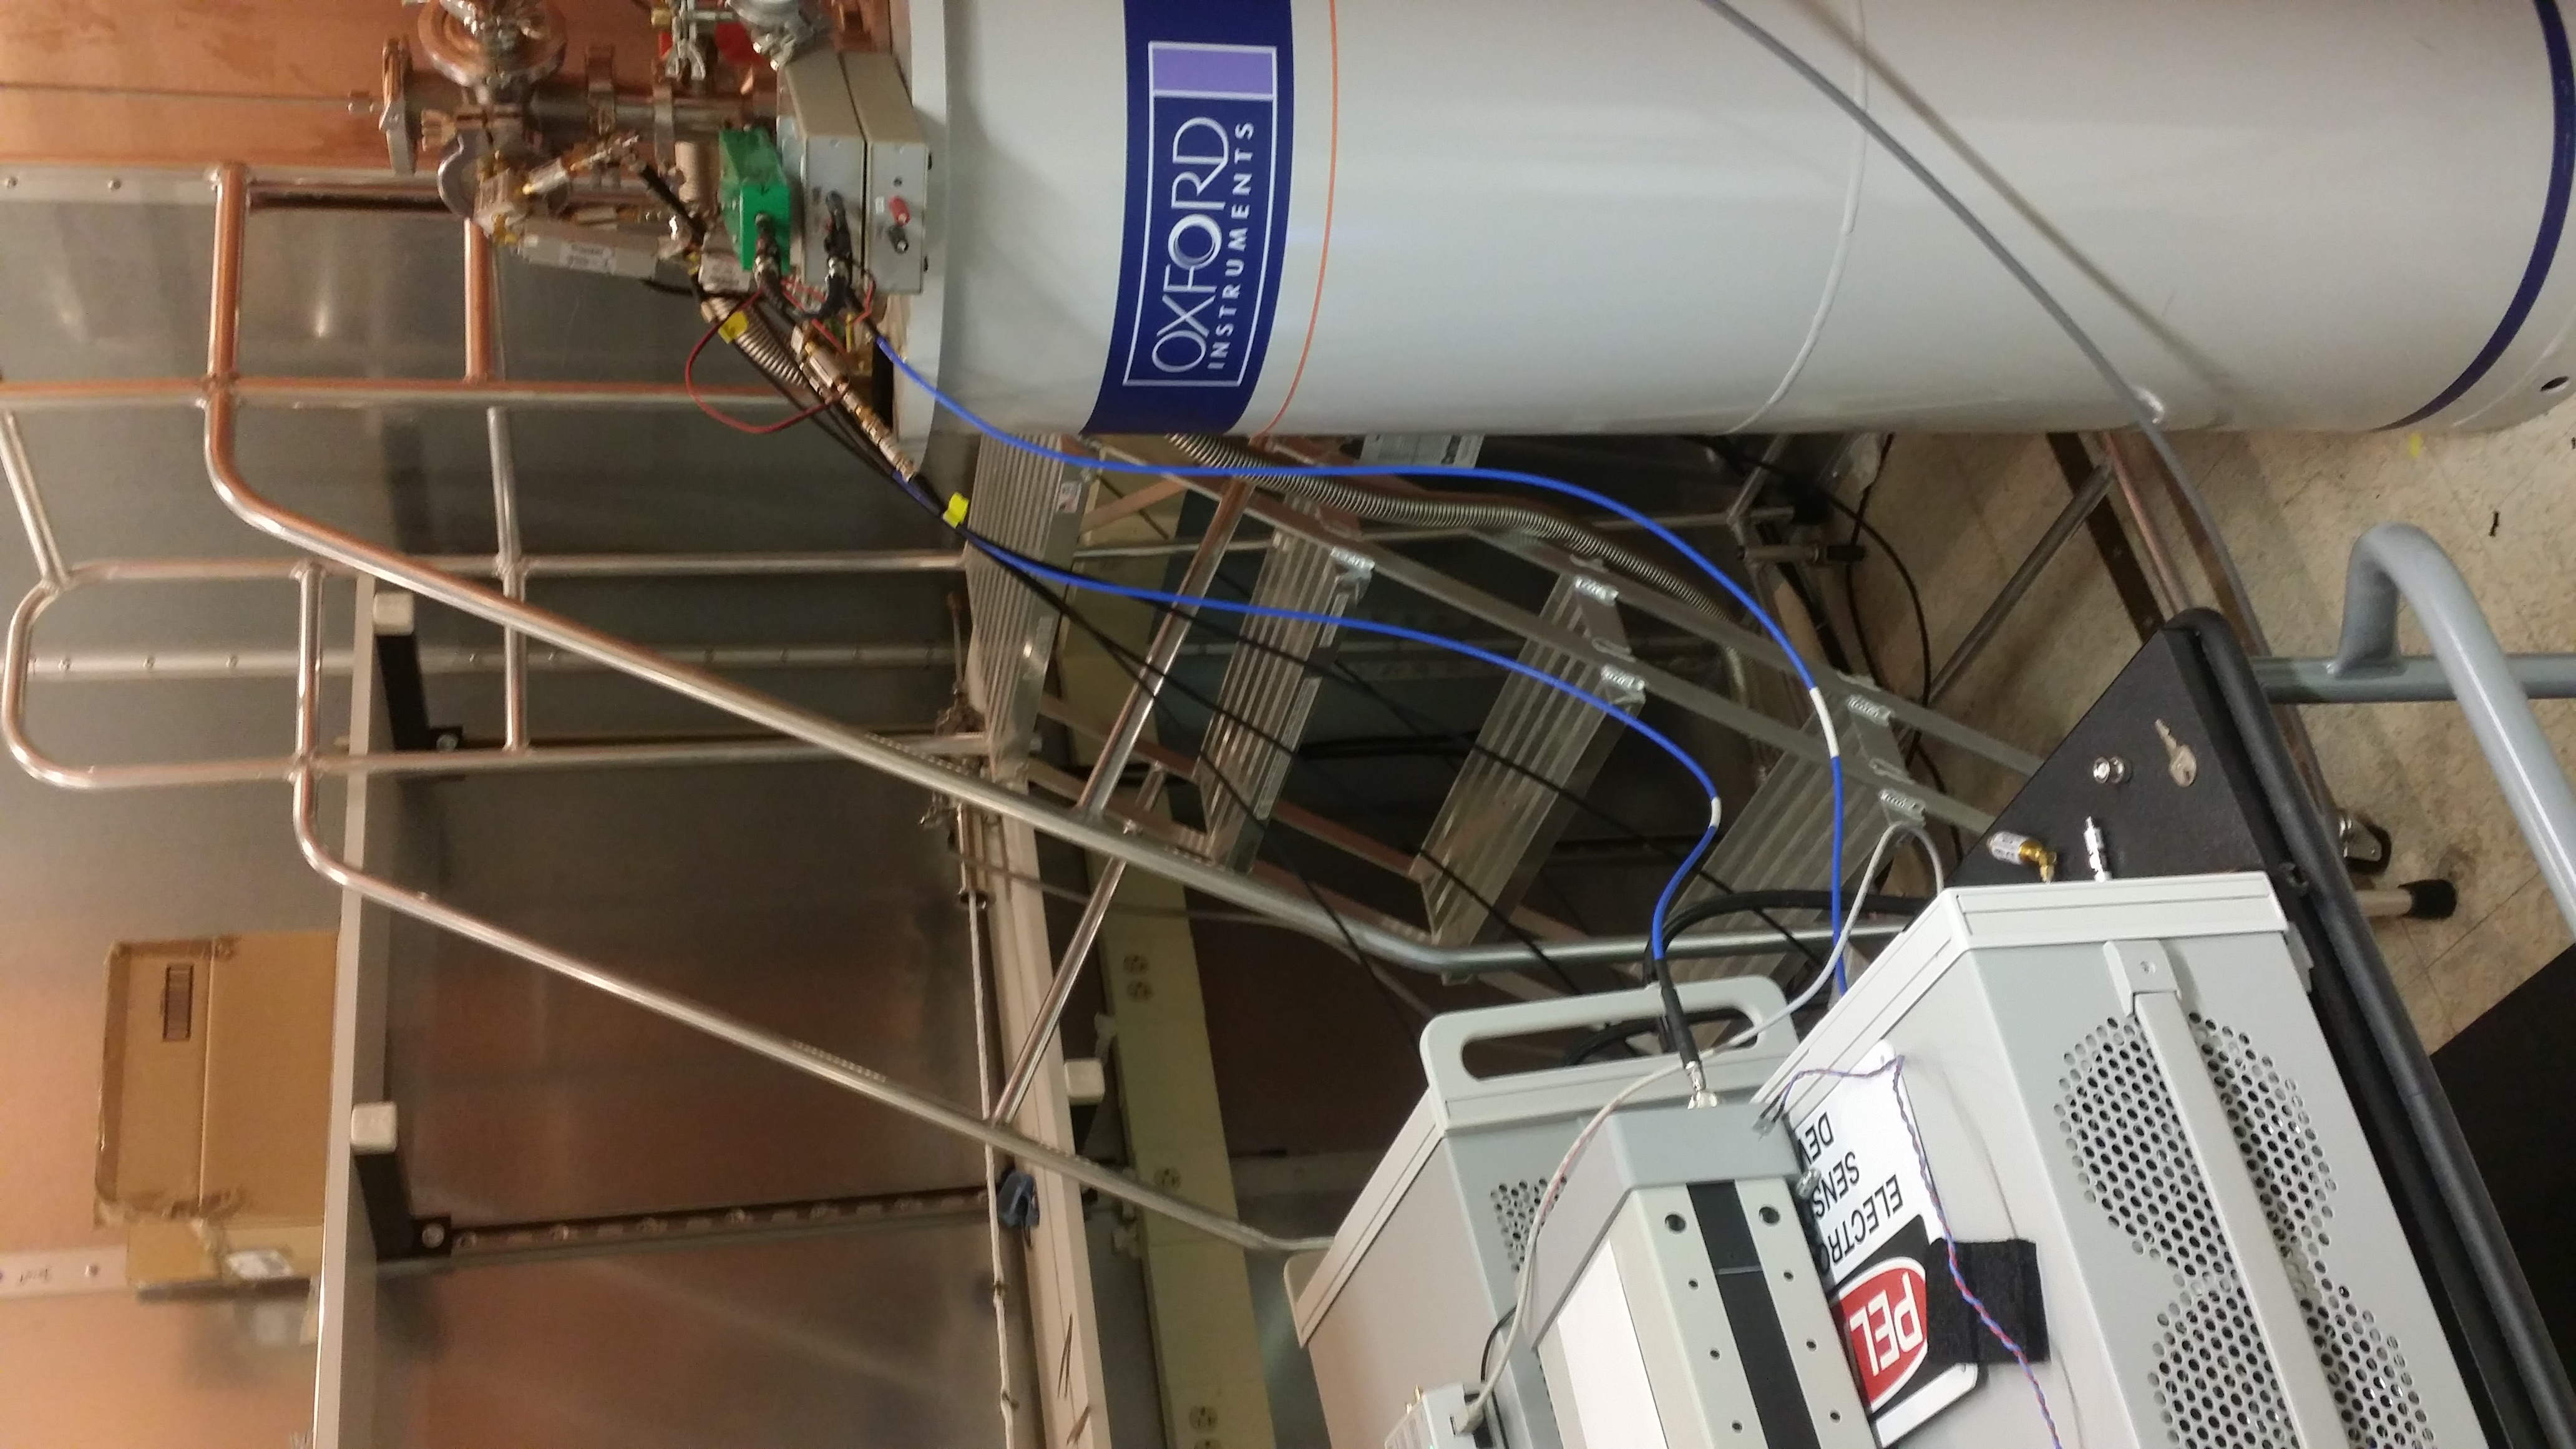
\includegraphics[angle=-90, width = 0.5\textwidth]{figures/appendix/cryostats/Oxford.jpg}
\caption{Image of the Oxford cryostat with VTI and RF probe during a measurement. All electronics are kept at room temperature. The entire fridge is housed inside a shielded metal room.}
\label{Fig:Appen:Oxford}
\end{figure}

As shown in Fig. \ref{Fig:Appen:Oxford}, once the sample is installed into sample package and mounted onto the RF probe, the entire unit can be lowered into the Oxford VTI. RF amplifiers can be placed either at low temperature or at room temperature just outside the fridge. For all experiments in this dissertation, all electronics were kept outside at room temperature.


\section{Leiden}
\begin{figure}
\centering
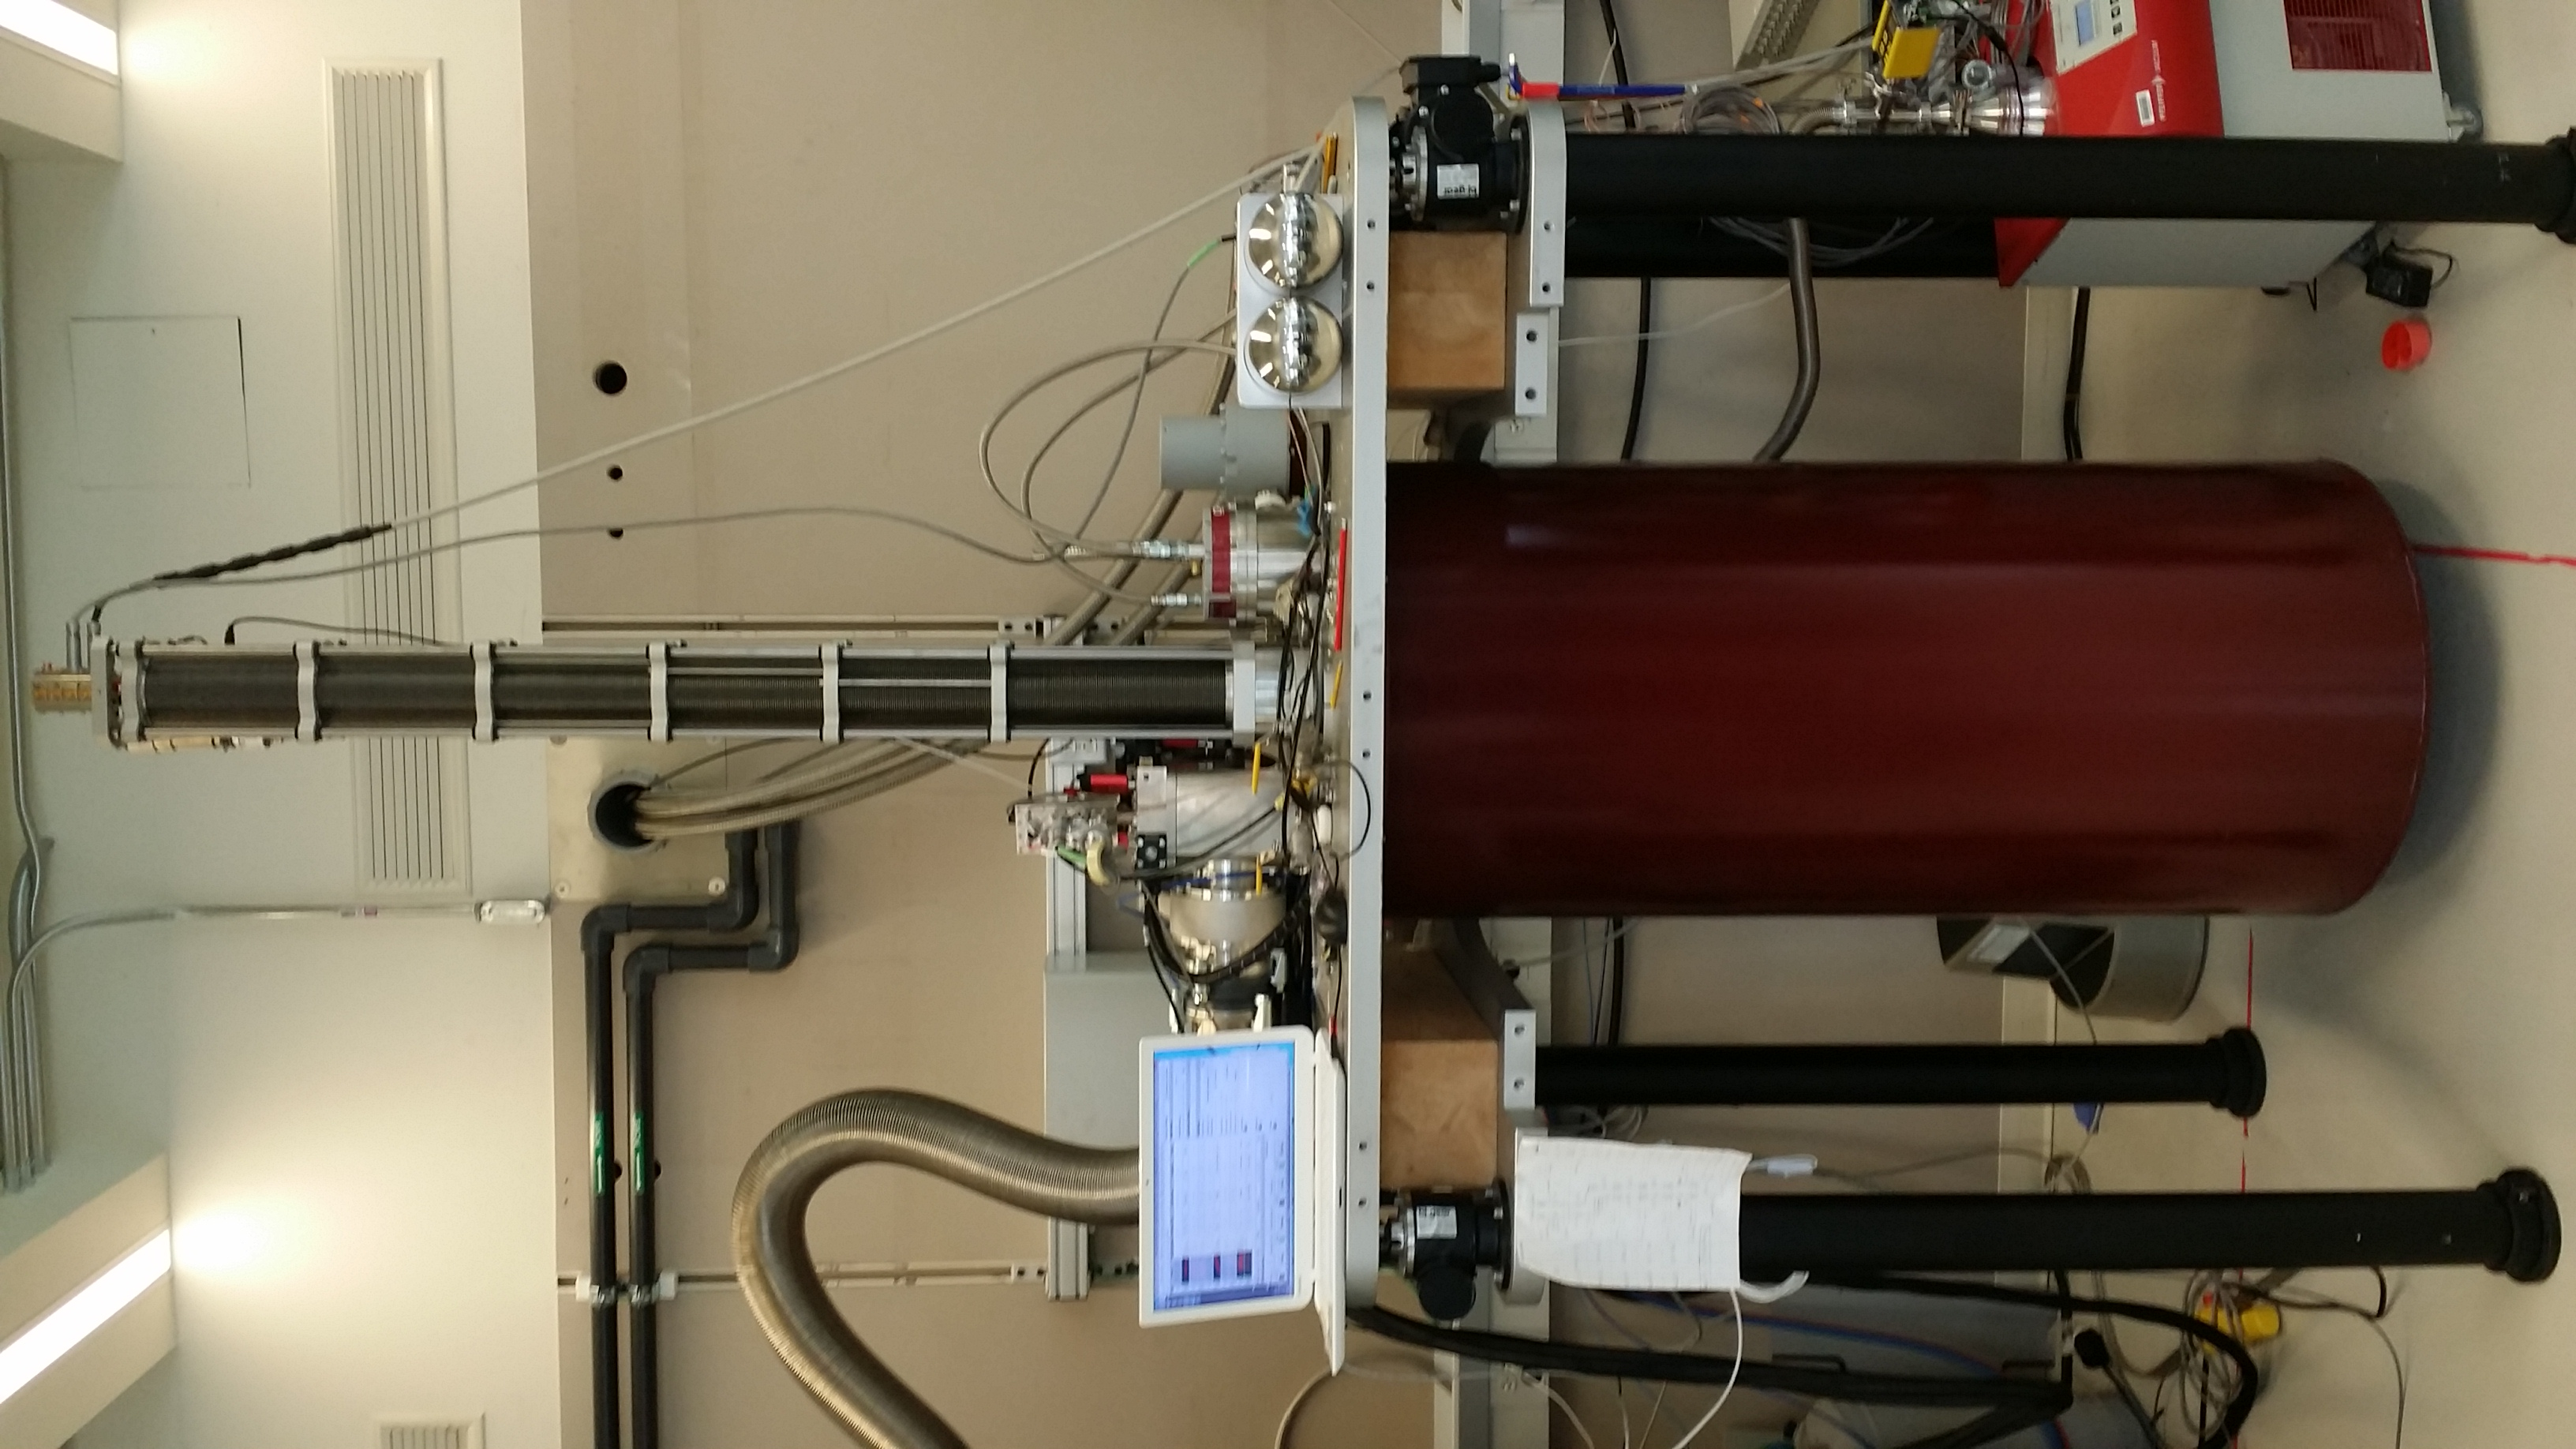
\includegraphics[angle=-90, width = 0.5\textwidth]{figures/appendix/cryostats/Leiden_closed.jpg}
\caption{Image of the closed cycle dilution refrigerator made by Leiden cryogenics installed in the Kim lab. The insertable, top-loading probe is seen in the upper half of the image enclosed in flexible bellows. The system sits on four electrically controlled, mechanical legs to lift the system for easy maintenance.}
\label{Fig:Appen:Leiden_closed}
\end{figure}

\newthought{For ultra-low temperature experiments}, a dry dilution refrigerator from Leiden cryogenics was used, as shown in Fig. \ref{Fig:Appen:Leiden_closed}. This entirely closed cycle system has a base temperature of ${\sim}10~mK$ and a large bore (${\sim}6$ inches) magnet with a maximum field strength of $5~T$. To facilitate fast experiment turn around times, it is equipped with a top loading probe which can bring a sample down to base temperature in a few hours. To access the cold plates for maintenance or install a longer term experimental setup, the fridge vacuum shields can be removed with the help of 4 electrically controlled, mechanical legs, as shown in Fig. \ref{Fig:Appen:Leiden_opening}.  

\begin{figure}
\centering
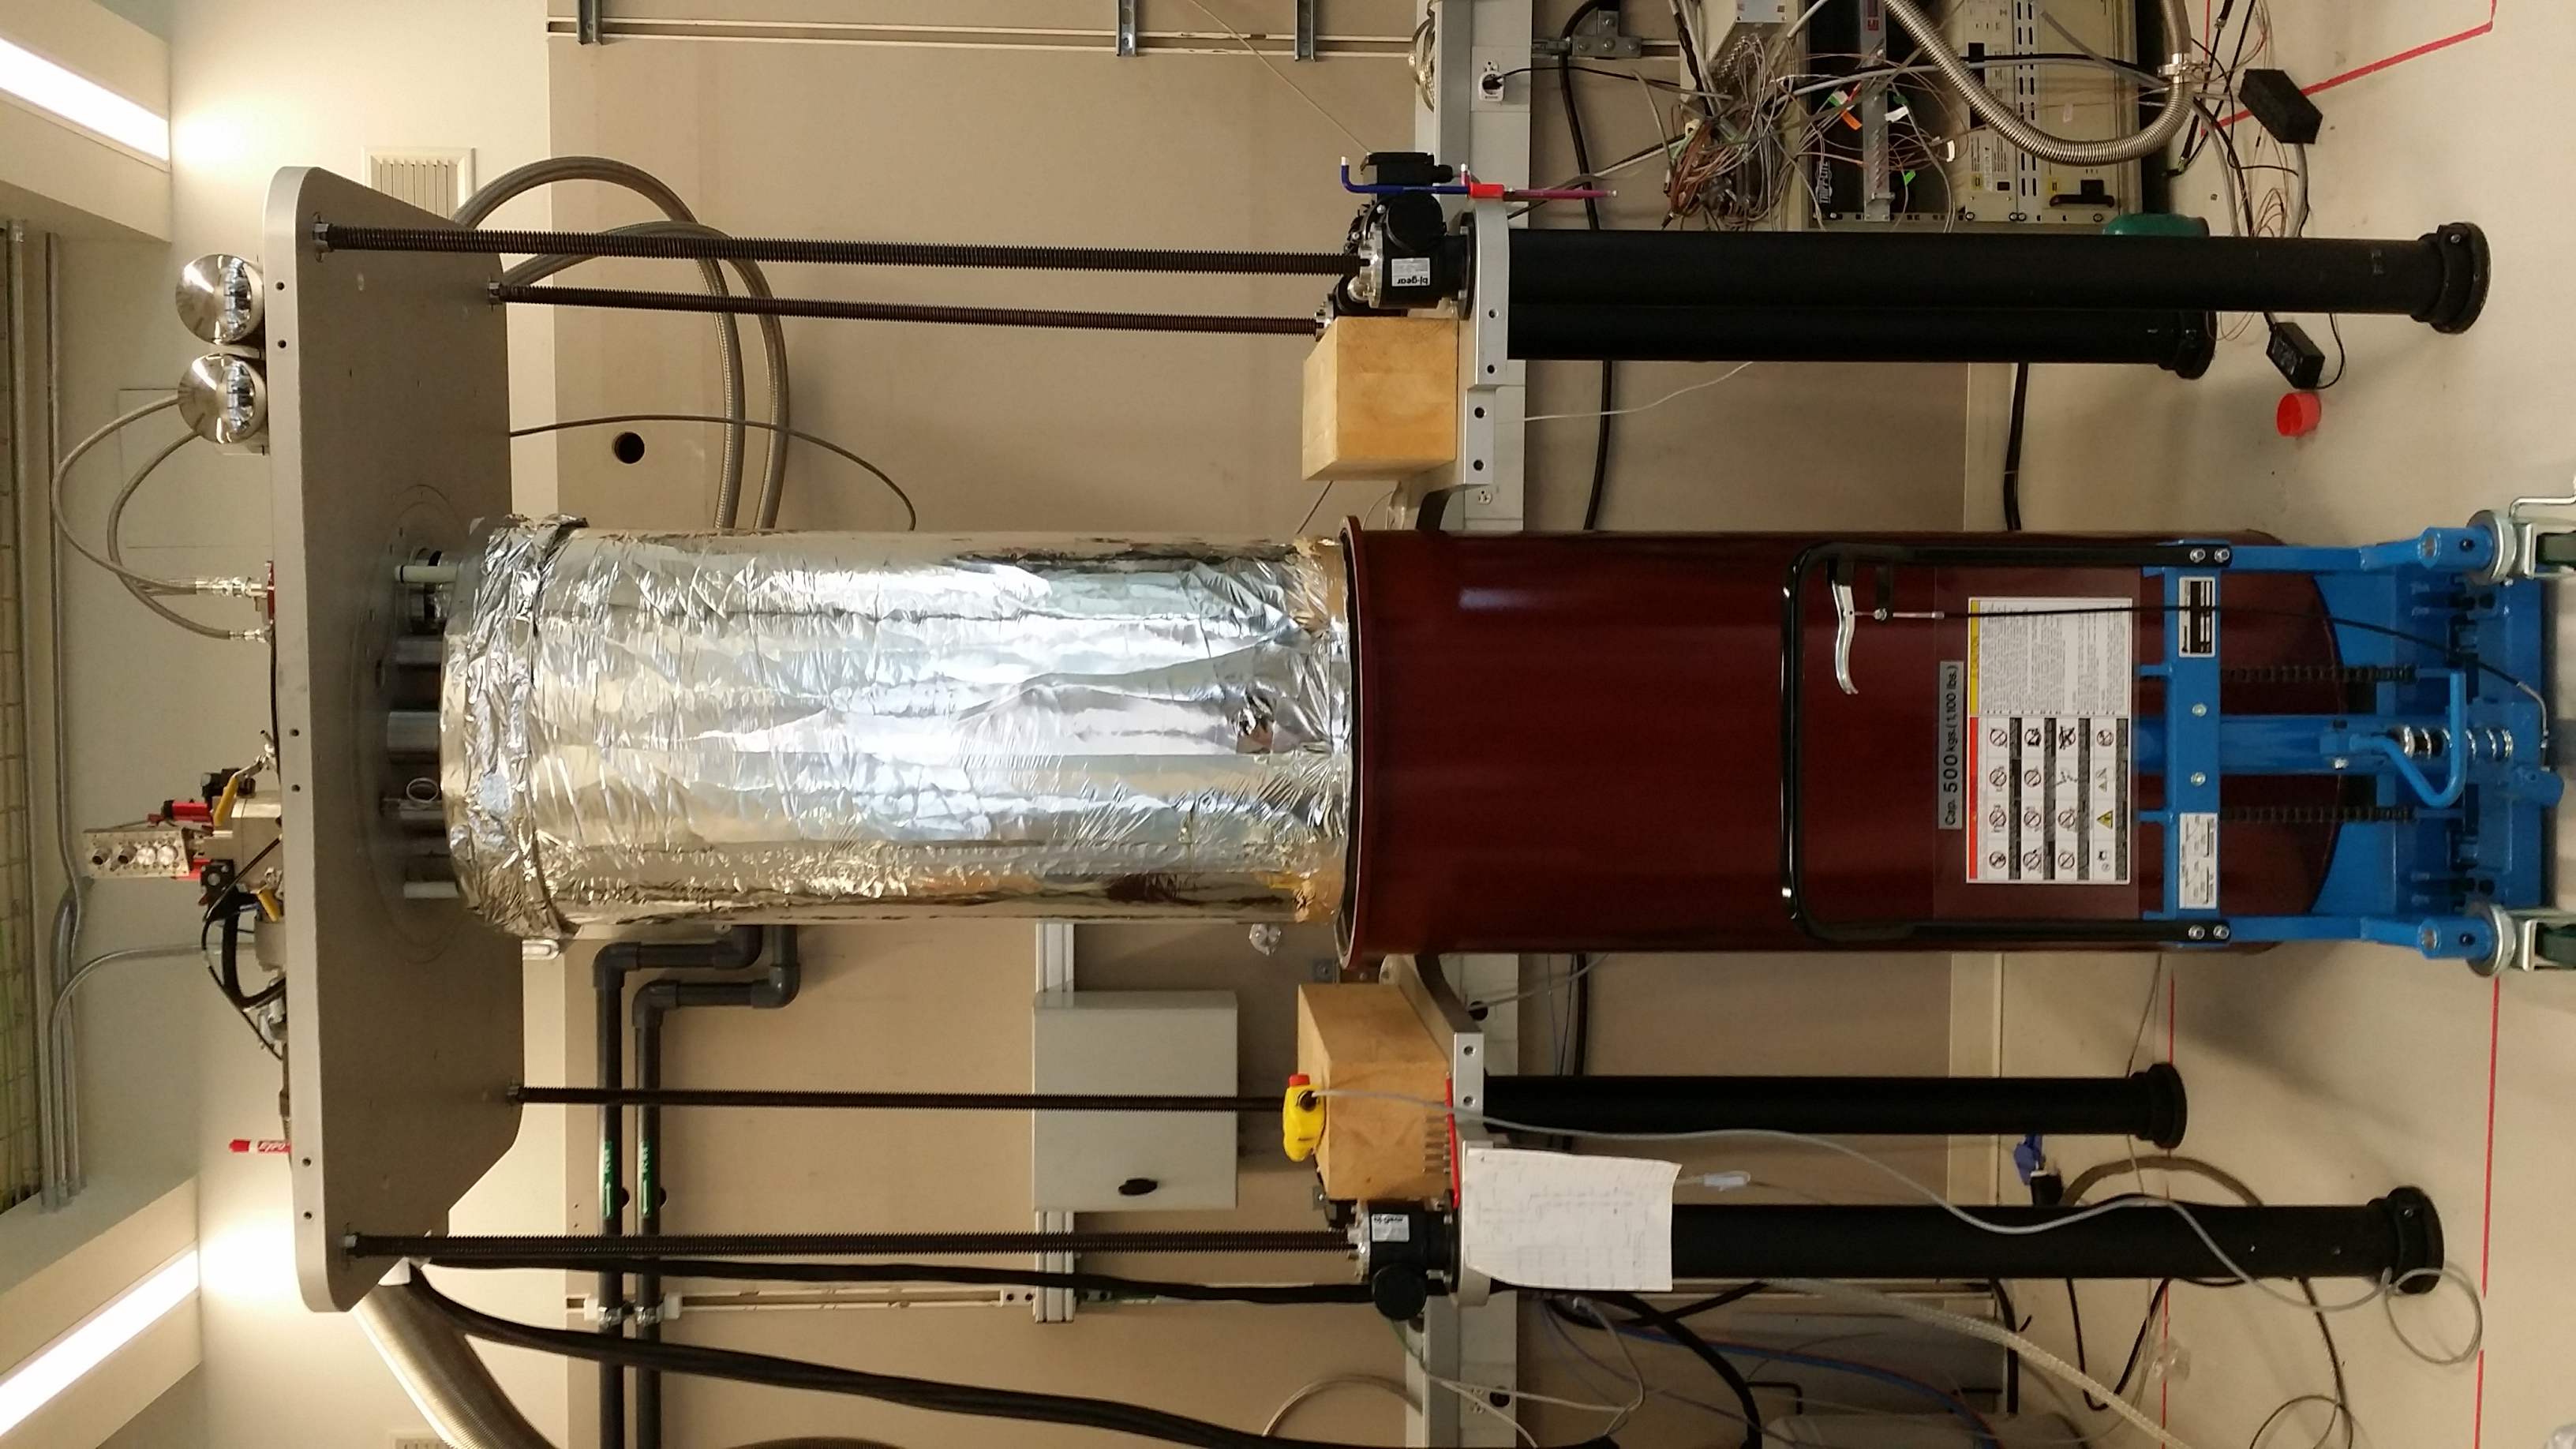
\includegraphics[angle=-90,width = 0.5\textwidth]{figures/appendix/cryostats/Leiden_opening.jpg}
\caption{Image of the Leiden cryostat being disassembled. The four electrically controlled legs are extended, lifting the entire system for easy maintenance.}
\label{Fig:Appen:Leiden_opening}
\end{figure}

Inside, the system consists of two independent vacuum chambers and five large gold plated copper plates thermally isolated from each other. The first and second plates are cooled by an electrically isolated pulse tube and, during operation, typically run at $50~K$ and $4-5~K$, respectively. The outer vacuum chamber (OVC) contains the entire $50~K$ plate and the upper half of the $4~K$ plate along with two sorption pumps and two heaters. The bottom half of the $4~K$ plate forms the top of the inner vacuum chamber (IVC) which is sealed with a Kapton o-ring. Four large SS tubes connect into the IVC to allow probes to enter; the central port is used for the main probe (described below), one of the secondary ports is used to bring in 16 RF coaxial cables, and the other two are held in reserve for future expansions. The bottom half of the $4~K$ plate also contains 2 sorption pumps which pump out the IVC and can be heated (via internal heaters) to release exchange gas into the IVC. The third plate contains the still/impedances and typically operates at a temperature of around $0.8~K$. The still has an on-board heater allowing the He mixture evaporation rate to be controlled\footnote{In principle, raising the evaporation rate results in more cooling power and a high base temperature but in practice the rate must be adjusted to find the proper balance for a given setup.}. The $5~T$ magnet is bolted onto the still plate and thus operates at the still temperature, as shown in Fig.~\ref{Fig:Appen:Leiden_magnet}.
\begin{figure}
\centering
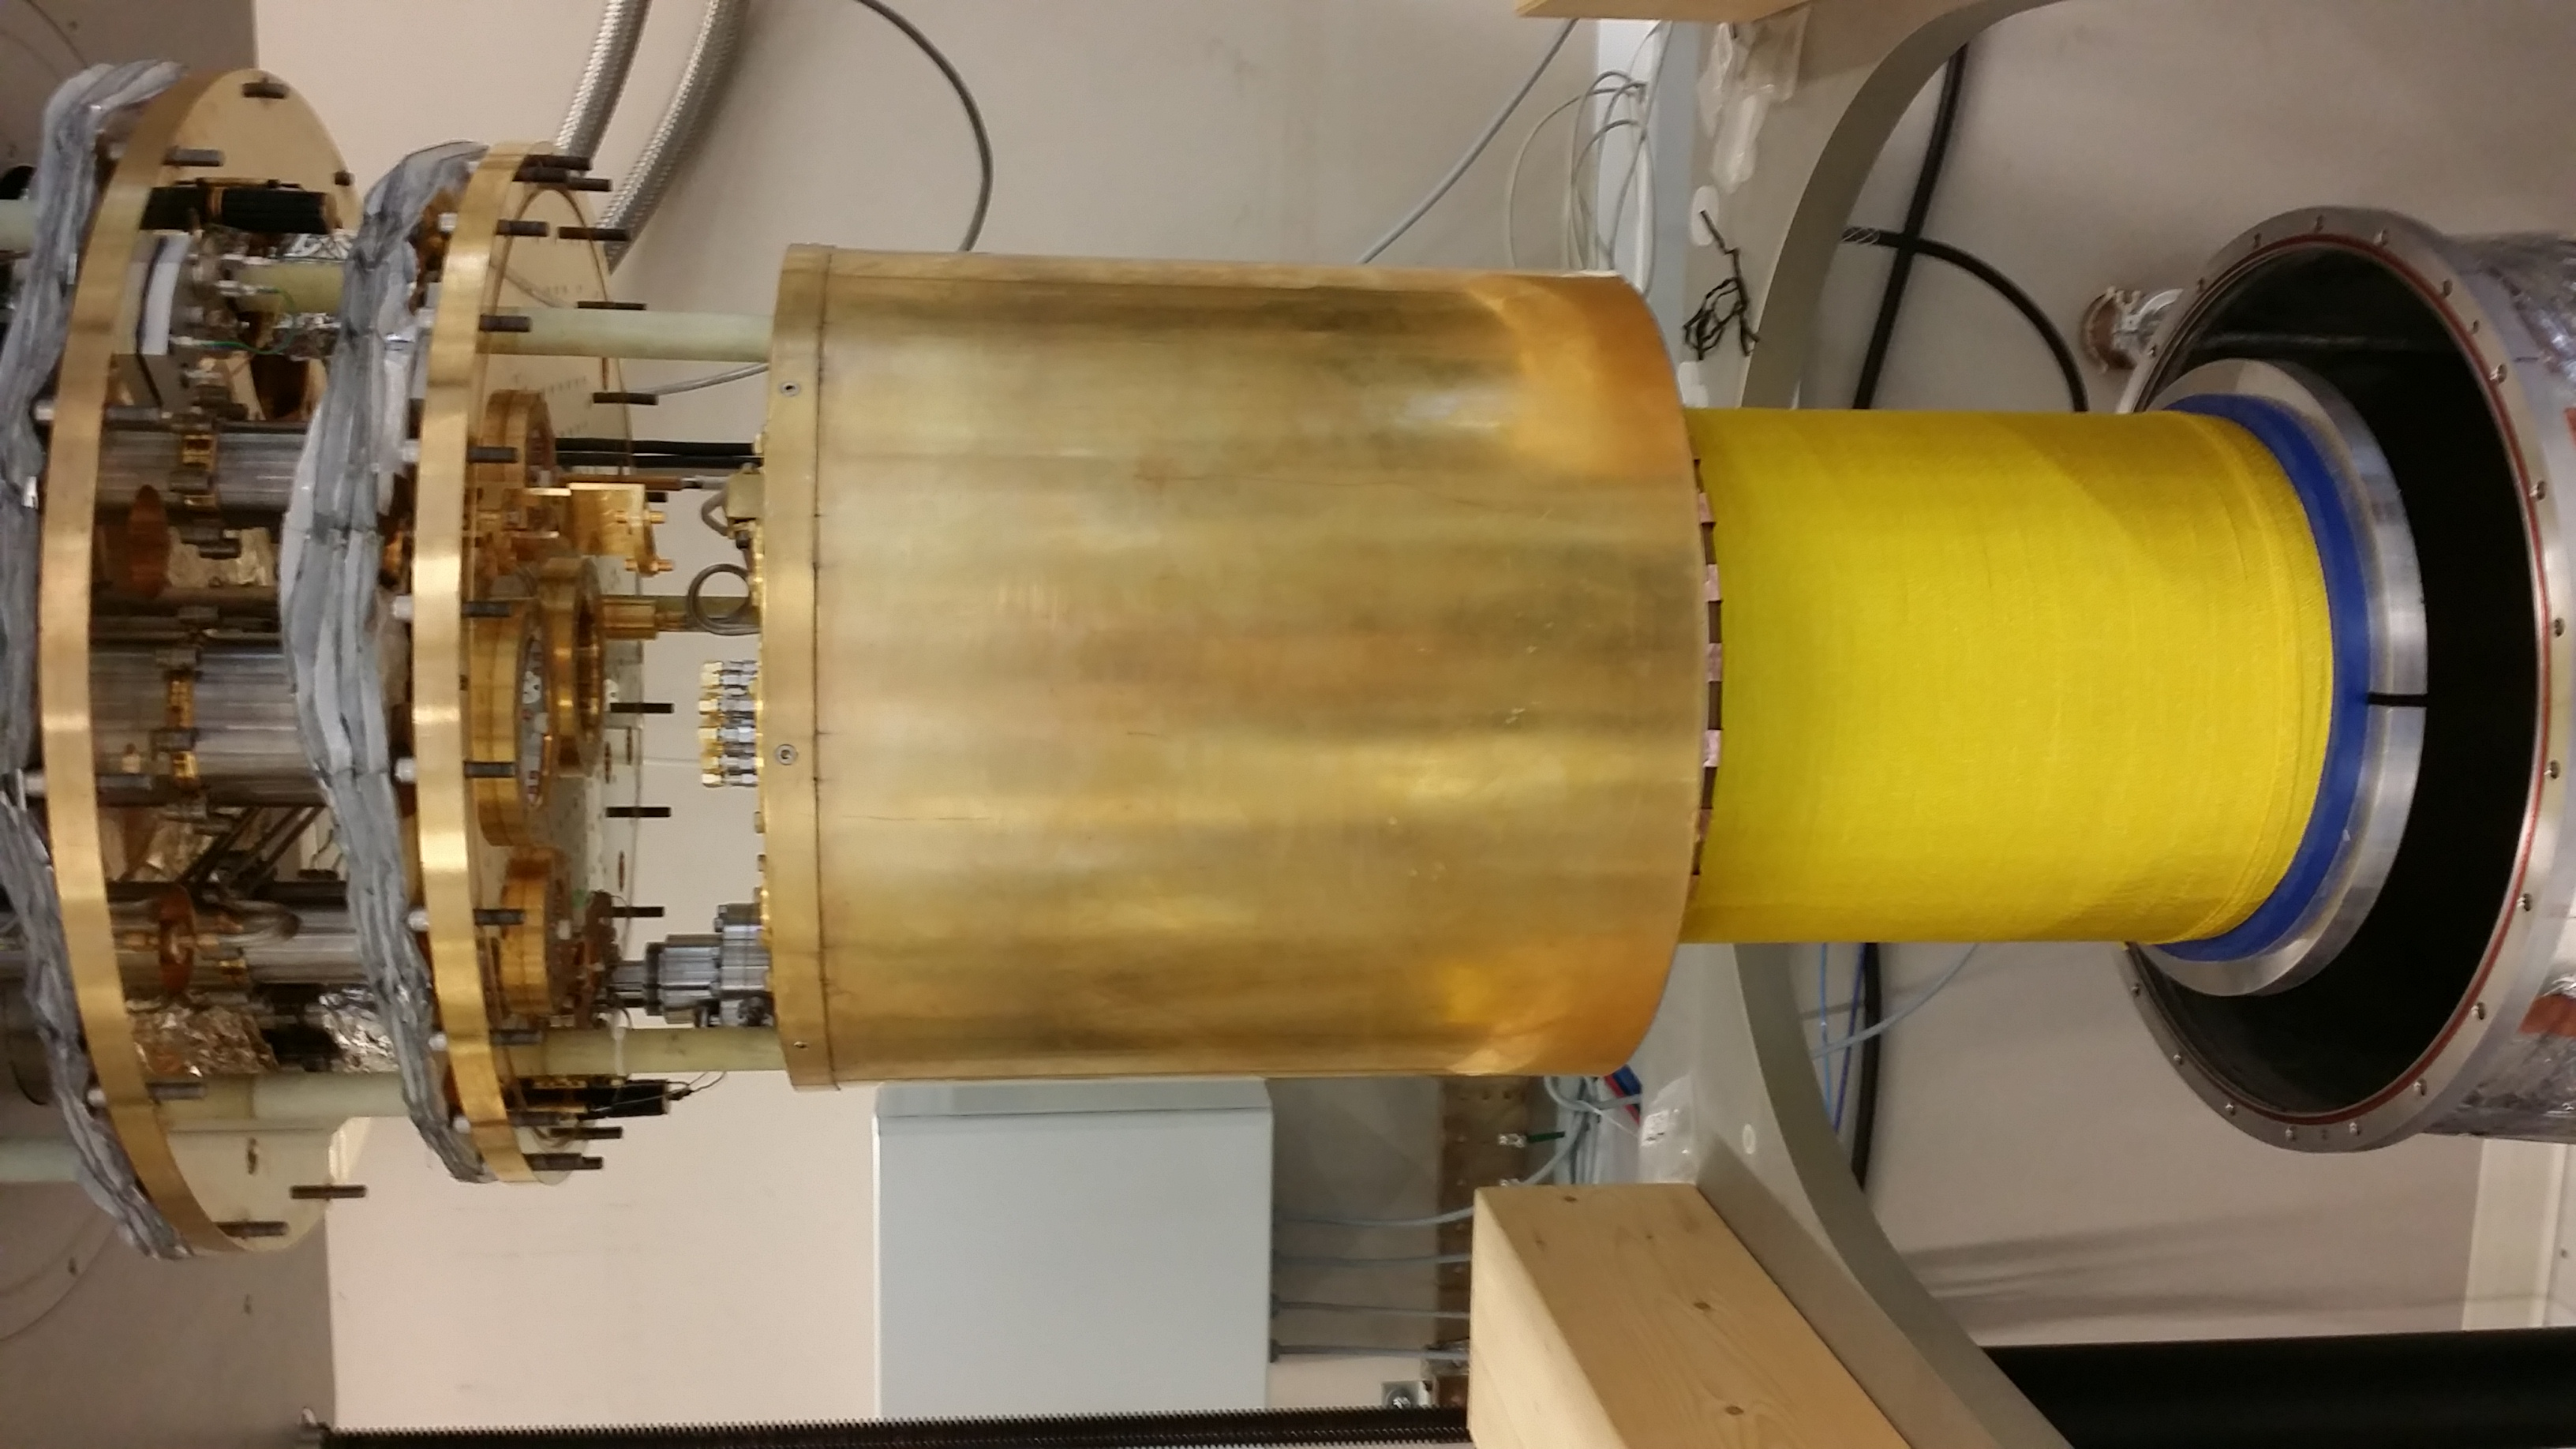
\includegraphics[angle=-90,width = 0.5\textwidth]{figures/appendix/cryostats/Leiden_magnet.jpg}
\caption{Image of the $5~T$ superconducting magnet, made by American Magnet Inc, installed in the Leiden system. The magnet is thermalized to the still plate and thus operates near $1~K$.}
\label{Fig:Appen:Leiden_magnet}
\end{figure}
 While running the magnet it is therefore import to watch the still temperature. The fourth plate has no direct cooling mechanism but serves as both a radiation shield and a location to mount the heat exchangers for the dilution circuit; during operation is typically sits around $100~mK$. The fifth and final plate contains the dilution mixing chamber and includes a long tail that dips into the magnet bore. Fig \ref{Fig:Appen:Leiden_Full} shown a close up of the entire IVC (lower 4 plates).

\begin{figure}
\centering
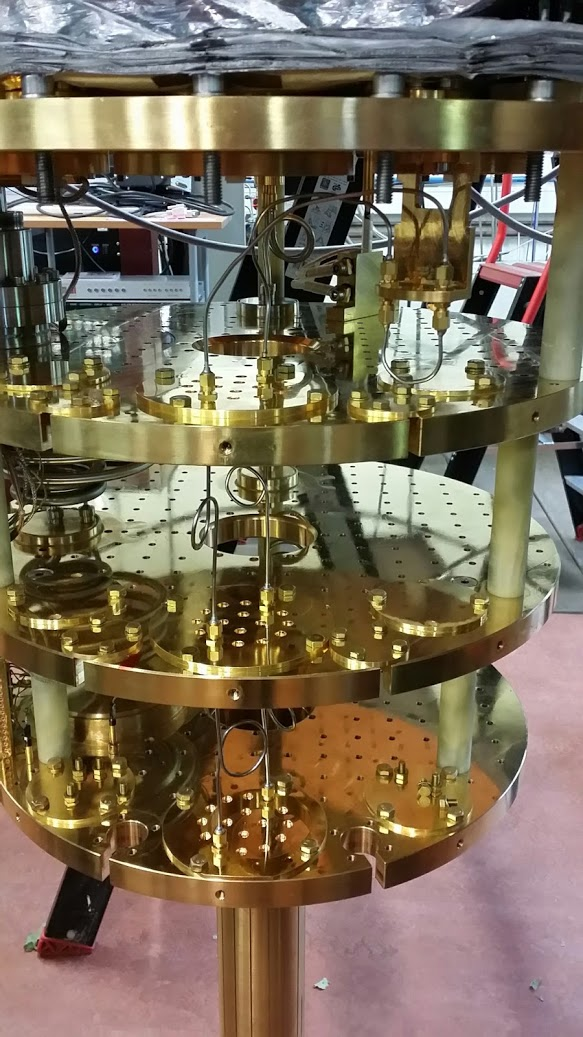
\includegraphics[width = 0.5\textwidth]{figures/appendix/cryostats/Leiden_full.jpg}
\caption{Close up of the Leiden IVC plates. Starting from the top, the shown plates are the $4~K$, still, $100~mK$, and mixing chamber plates. The still is the silver piece seen on the left side of the image mounted on the top side of the still plate. Image taken in Leiden, Netherlands while constructing the fridge. At the bottom of the image, the ``tail" that extends down into the magnet bore can be seen}
\label{Fig:Appen:Leiden_Full}
\end{figure}

To perform RF measurements, one of two options is available: firstly, if the number of cold microwave elements is small, all circuitry can be installed directly onto the insertable probe\footnote{The cooling power of the probe is limited by the thermal contact to the cold plates so caution must be taken if active elements such as amplifiers are required.}, secondly, the microwave components can be installed into the main body of the fridge and connected to the sample via internal lines and an RF ``clicking mechanism" that couples to the probe. As shown in Fig.~\ref{Fig:Appen:Leiden_lines}, internally microwaves lines connect each stage; 14 coaxial excitation lines with copper/nickel alloy inner and outer conductors and 2 measurement lines with superconducting niobium-titanium inner and outer conductors run between the stages. All excitation lines are attenuated at each stage to thermalize the electronic temperature (reduce the Johnson noise to the appropriate level).

\begin{figure}
\centering
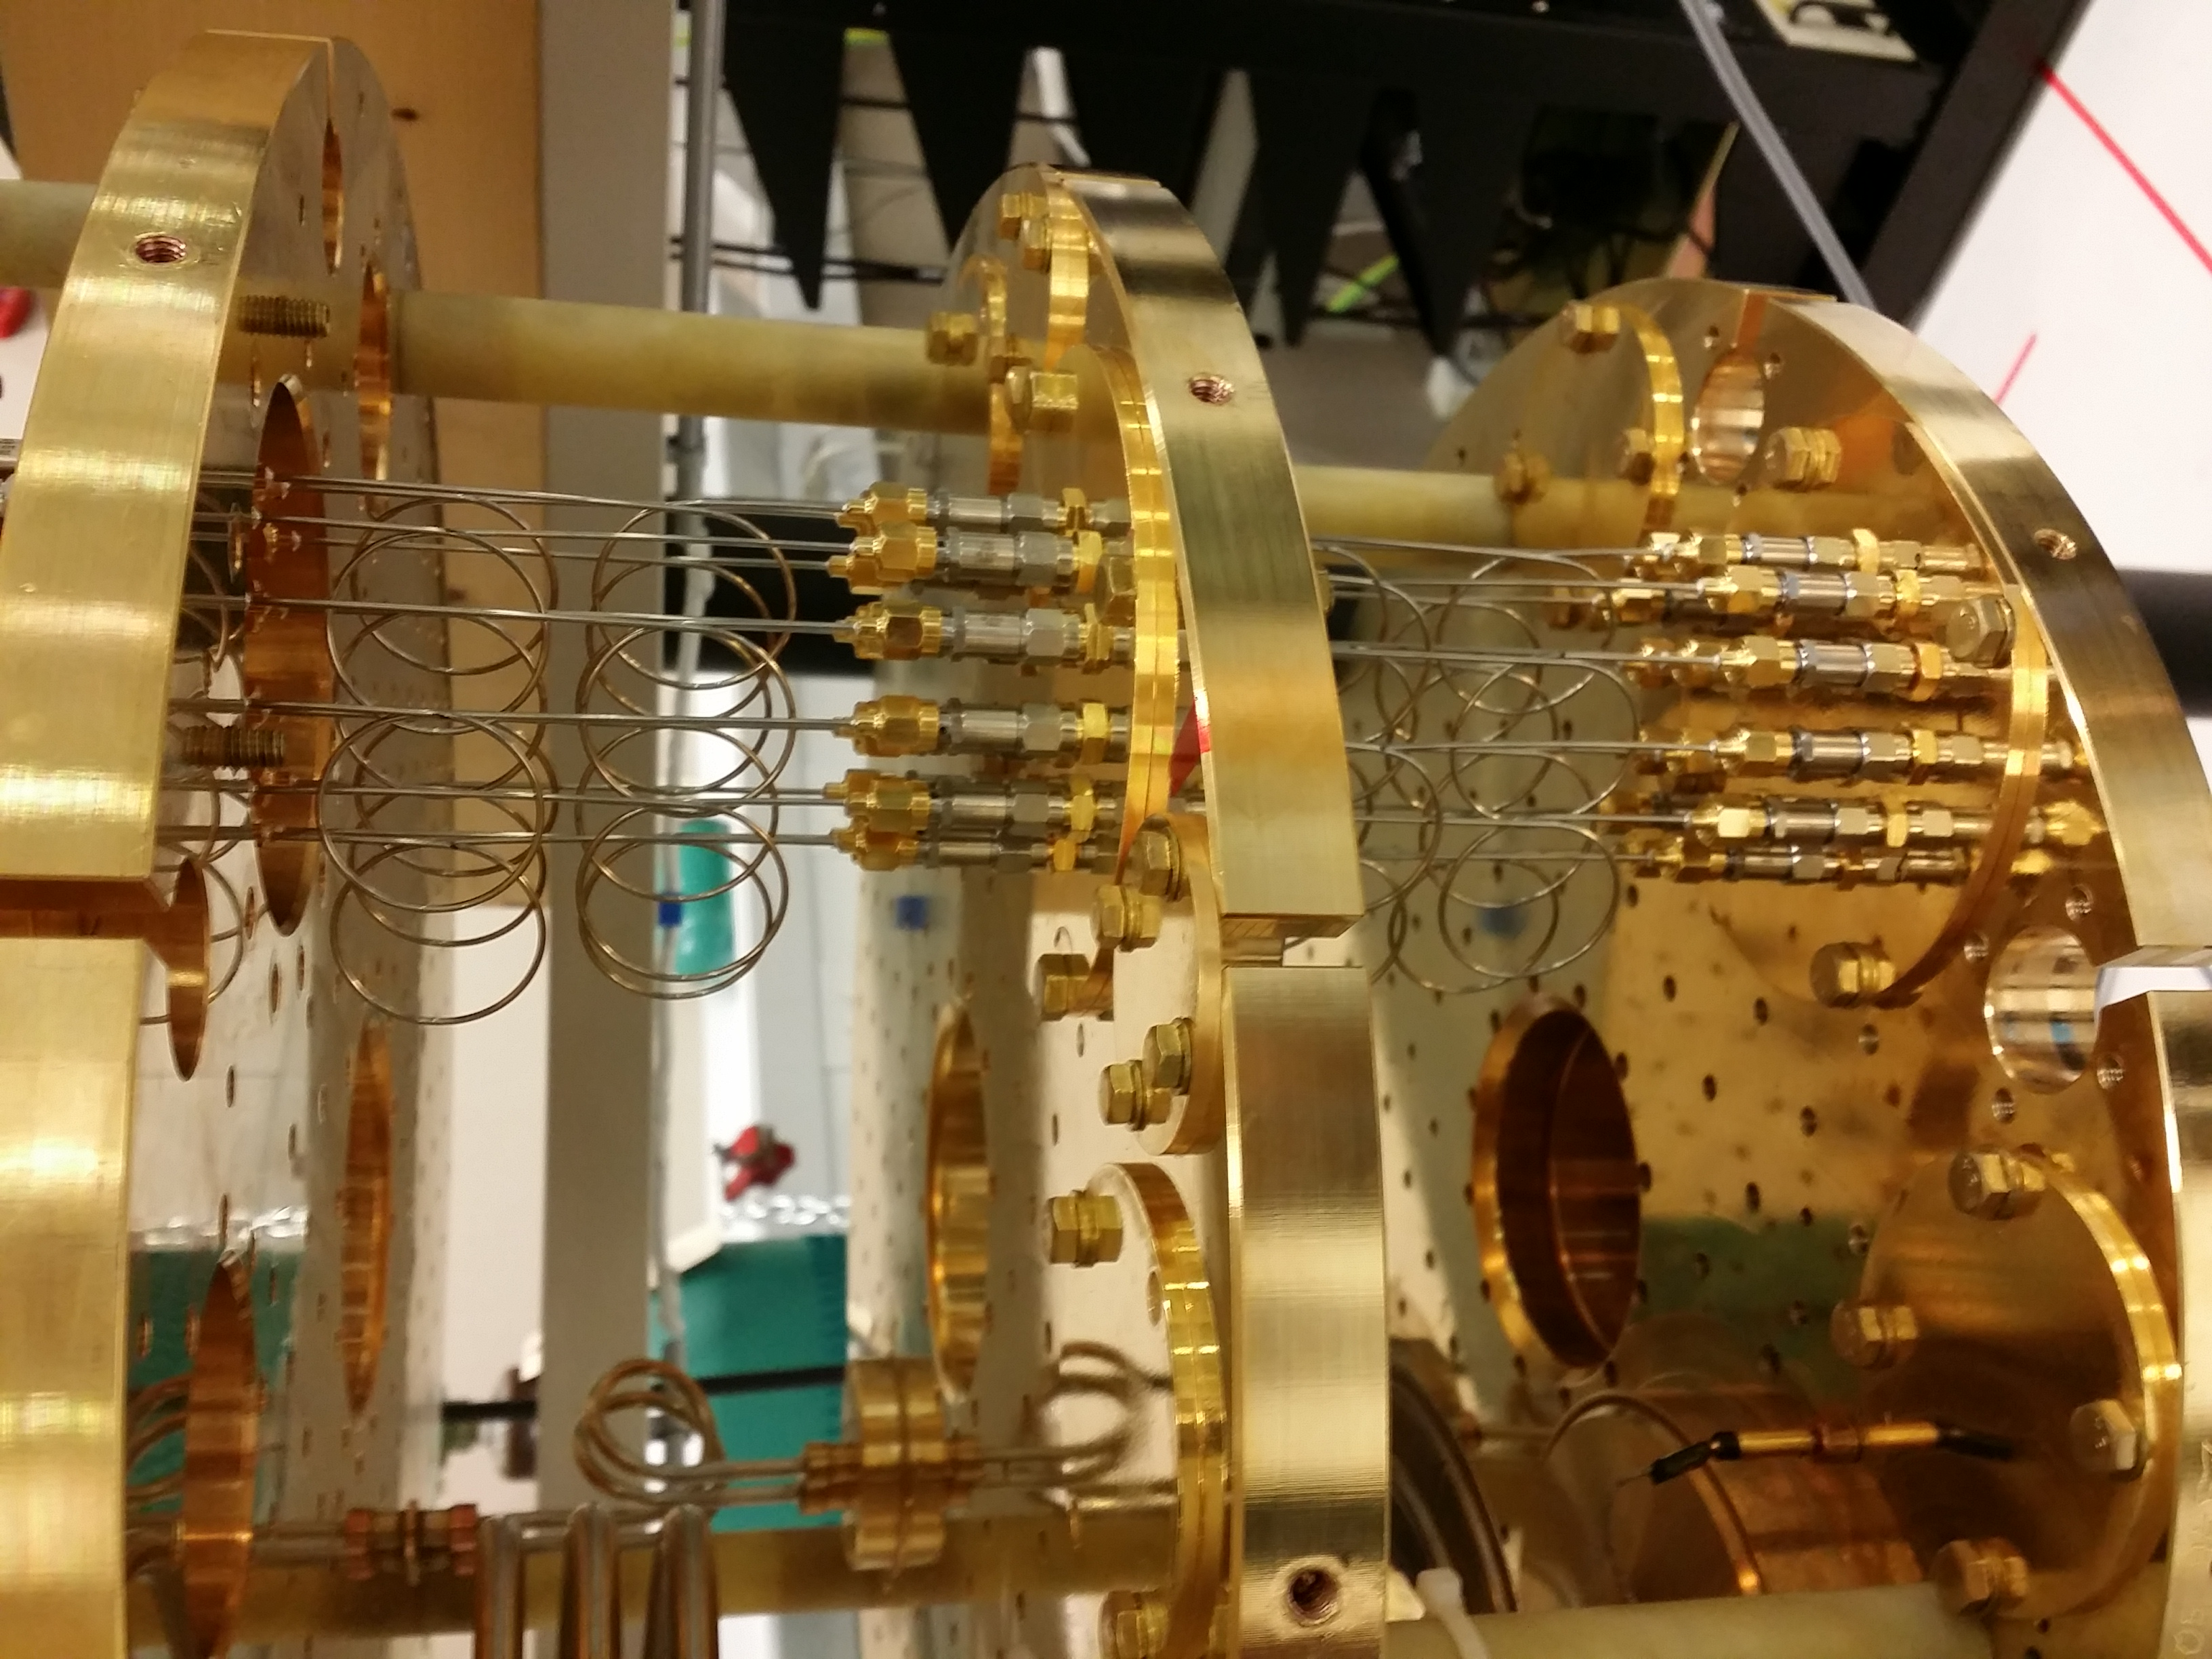
\includegraphics[angle=-90,width = 0.5\textwidth]{figures/appendix/cryostats/Leiden_lines.jpg}
\caption{Image of the microwave lines inside in the body of the Leiden cryostat. Shown here are the 14 excitation lines connecting the still plate to the mixing chamber plate attenuated at every stage. Not shown are the 2 superconducting measurement lines installed alongside these without attenuators.}
\label{Fig:Appen:Leiden_lines}
\end{figure}

The insertable, top-loaded probe is shown in Fig.~\ref{Fig:Appen:Leiden_bellows_open} with the electronically controlled bellows lowered. The probe holds up to 8 high frequency lines and over 24 DC lines if needed. For each of the five temperature stages in the main fridge body, the probe has a corresponding set of pneumatic expanding thermalization plates; once the probe is fully inserted, these plates expand to thermally sink each stage of the insert to a stage in the main body\footnote{While most stages sink well, the $50~K$ stage is in the OVC and therefore has to thermalize through a SS tube.}. A location to place 8 SMA bulkheads is built into every temperature stage. Attached to the final (mixing chamber) stage in a long extension arm which reaches into the magnet bore. The sample is placed at the end of this extender. 
\begin{figure}
\centering
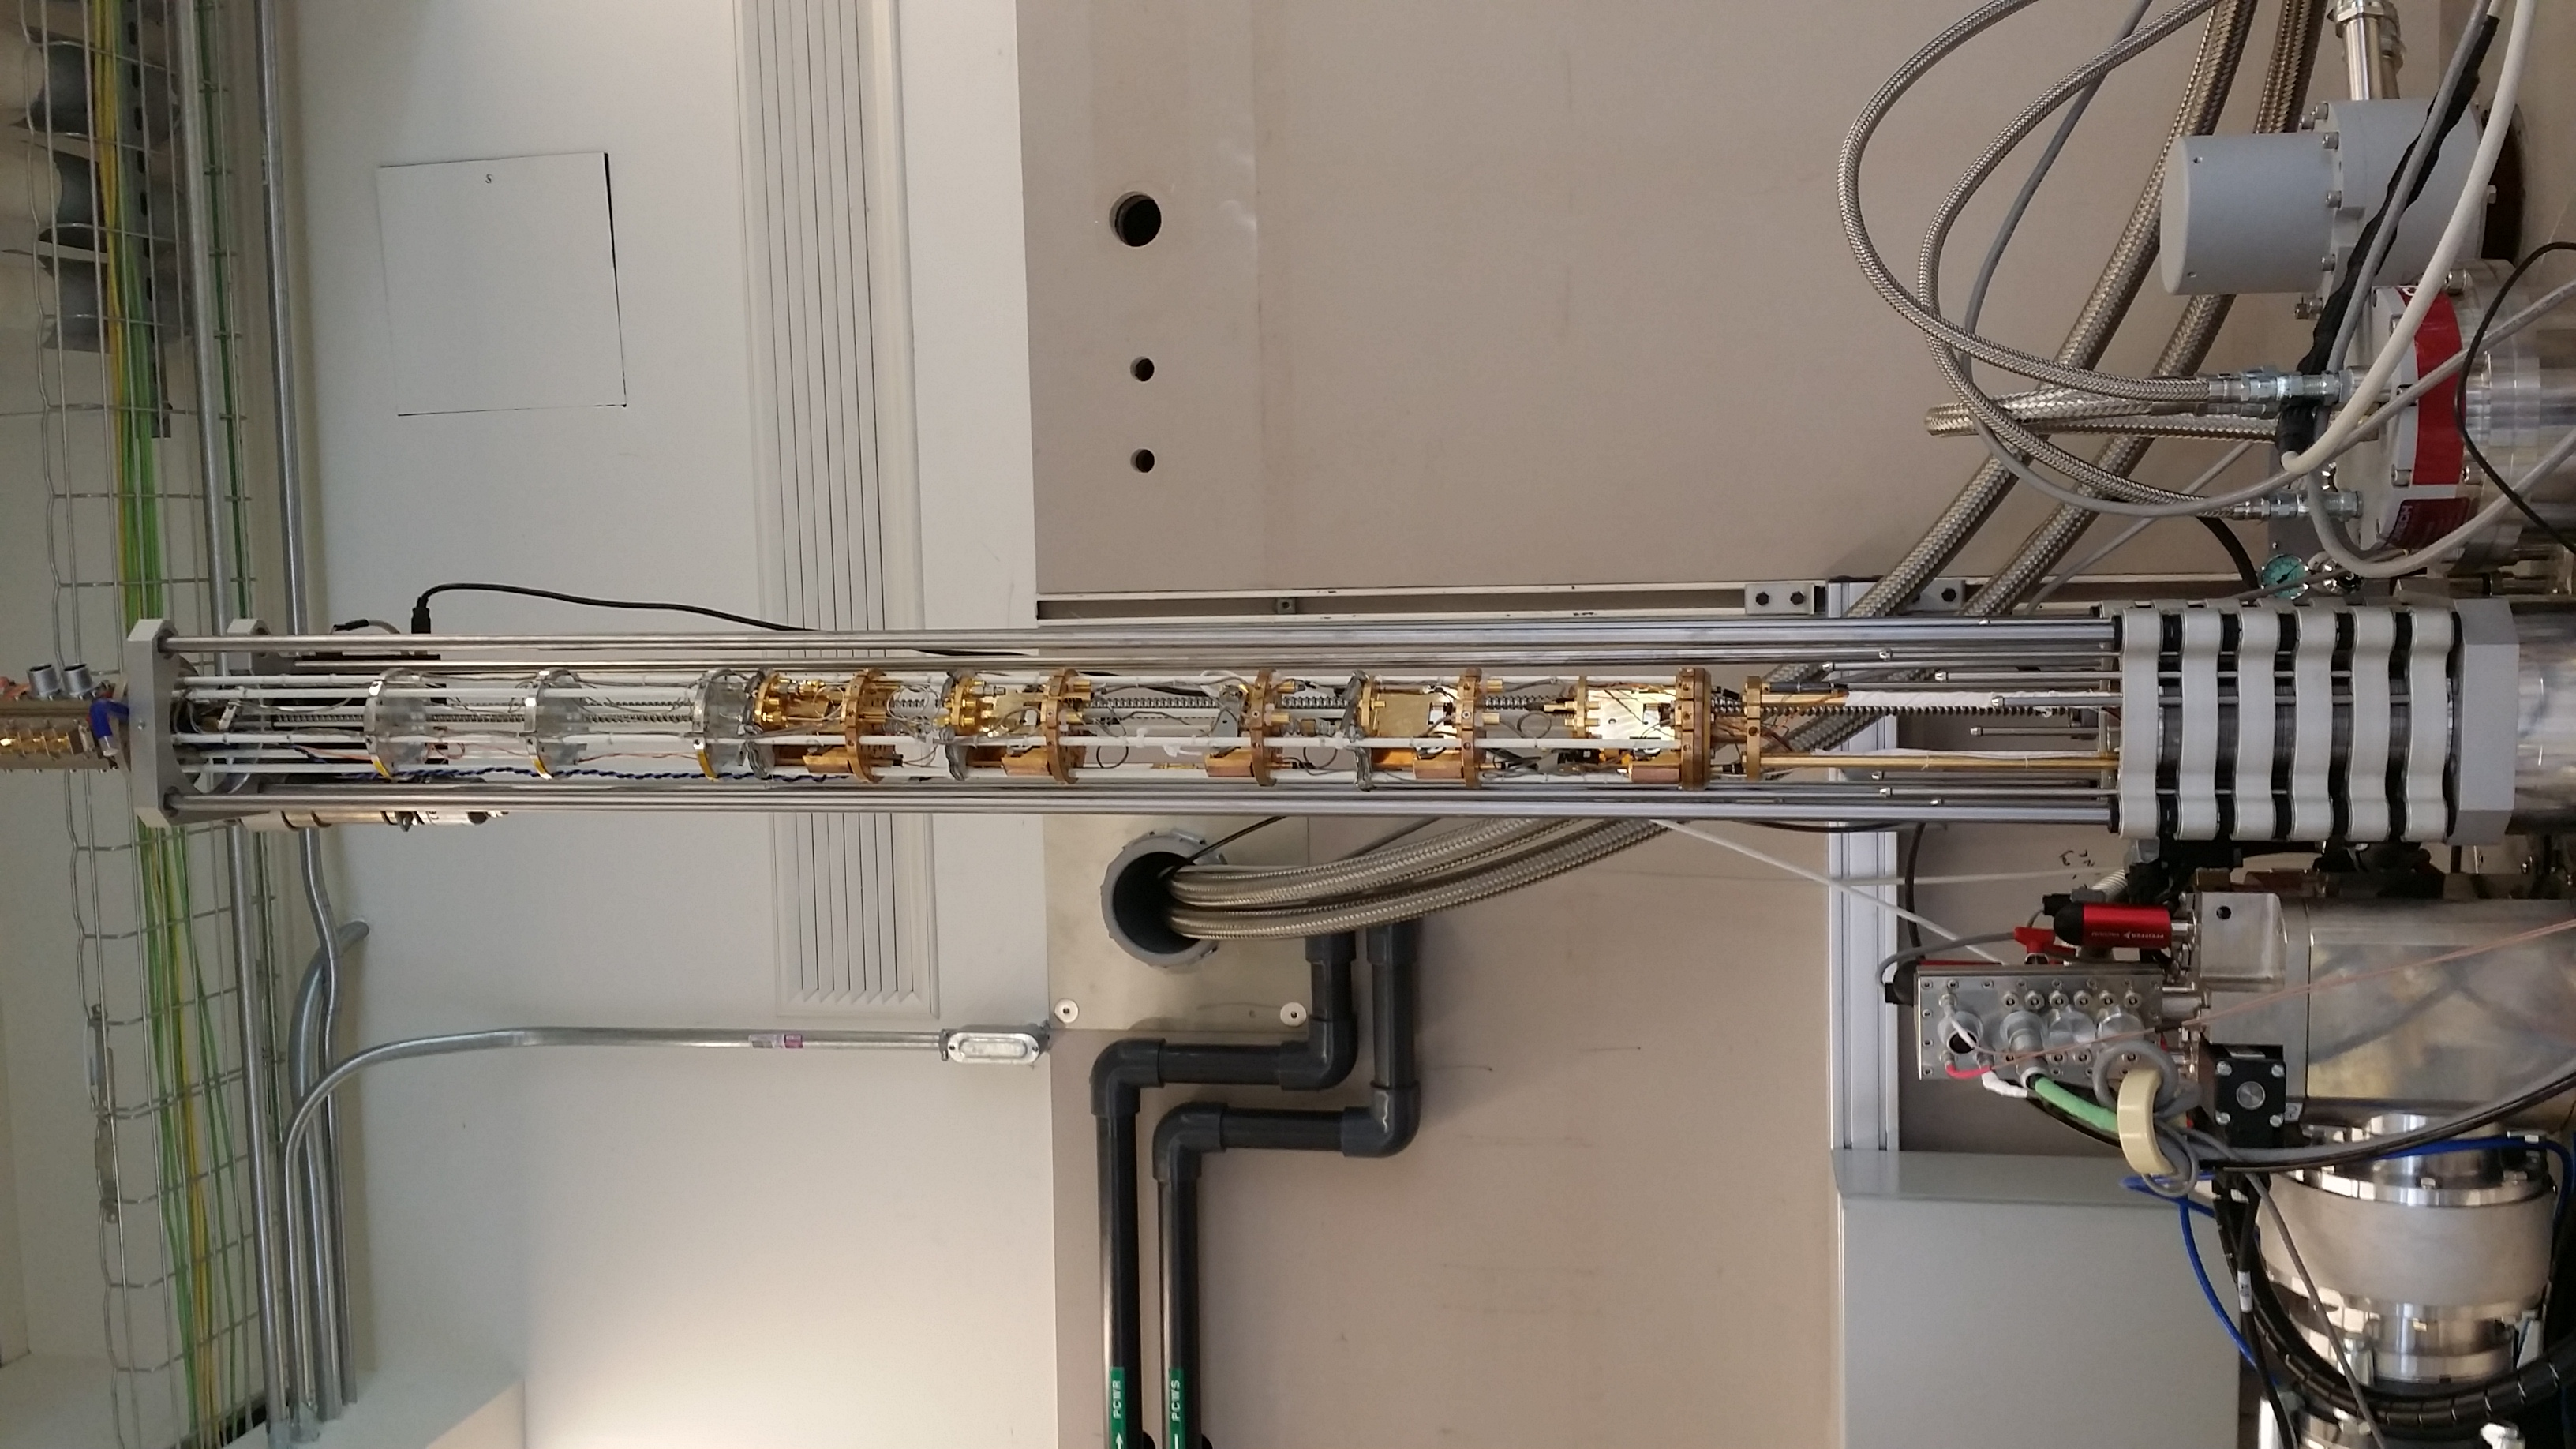
\includegraphics[angle=-90,width = 0.5\textwidth]{figures/appendix/cryostats/Leiden_bellows_open.jpg}
\caption{Image of the insertable, top-loading probe built for the Leiden dilution refrigerator with the retractable bellows lowered. Each gold plated copper section mechanically expands once inserted to thermalize to a stage in the main fridge body. Near the bottom of the probe, and extender is seen which, during operation, contains the sample and is lowered into the magnet bore.}
\label{Fig:Appen:Leiden_bellows_open}
\end{figure}

For the experiment in this dissertation, the number of cold microwave elements was small and thus all components could be installed onto the probe itself. Fig.~\ref{Fig:Appen:Leiden_probe} shows an example of one the these circuits. A cold amplifier\footnote{Cal-Tech CITLF$3$} is mounted to the $4~K$ stage and a bias-tee along with two directional couples are attached to allow for DC transport and RF reflection/gain measurements.

\begin{figure}
\centering
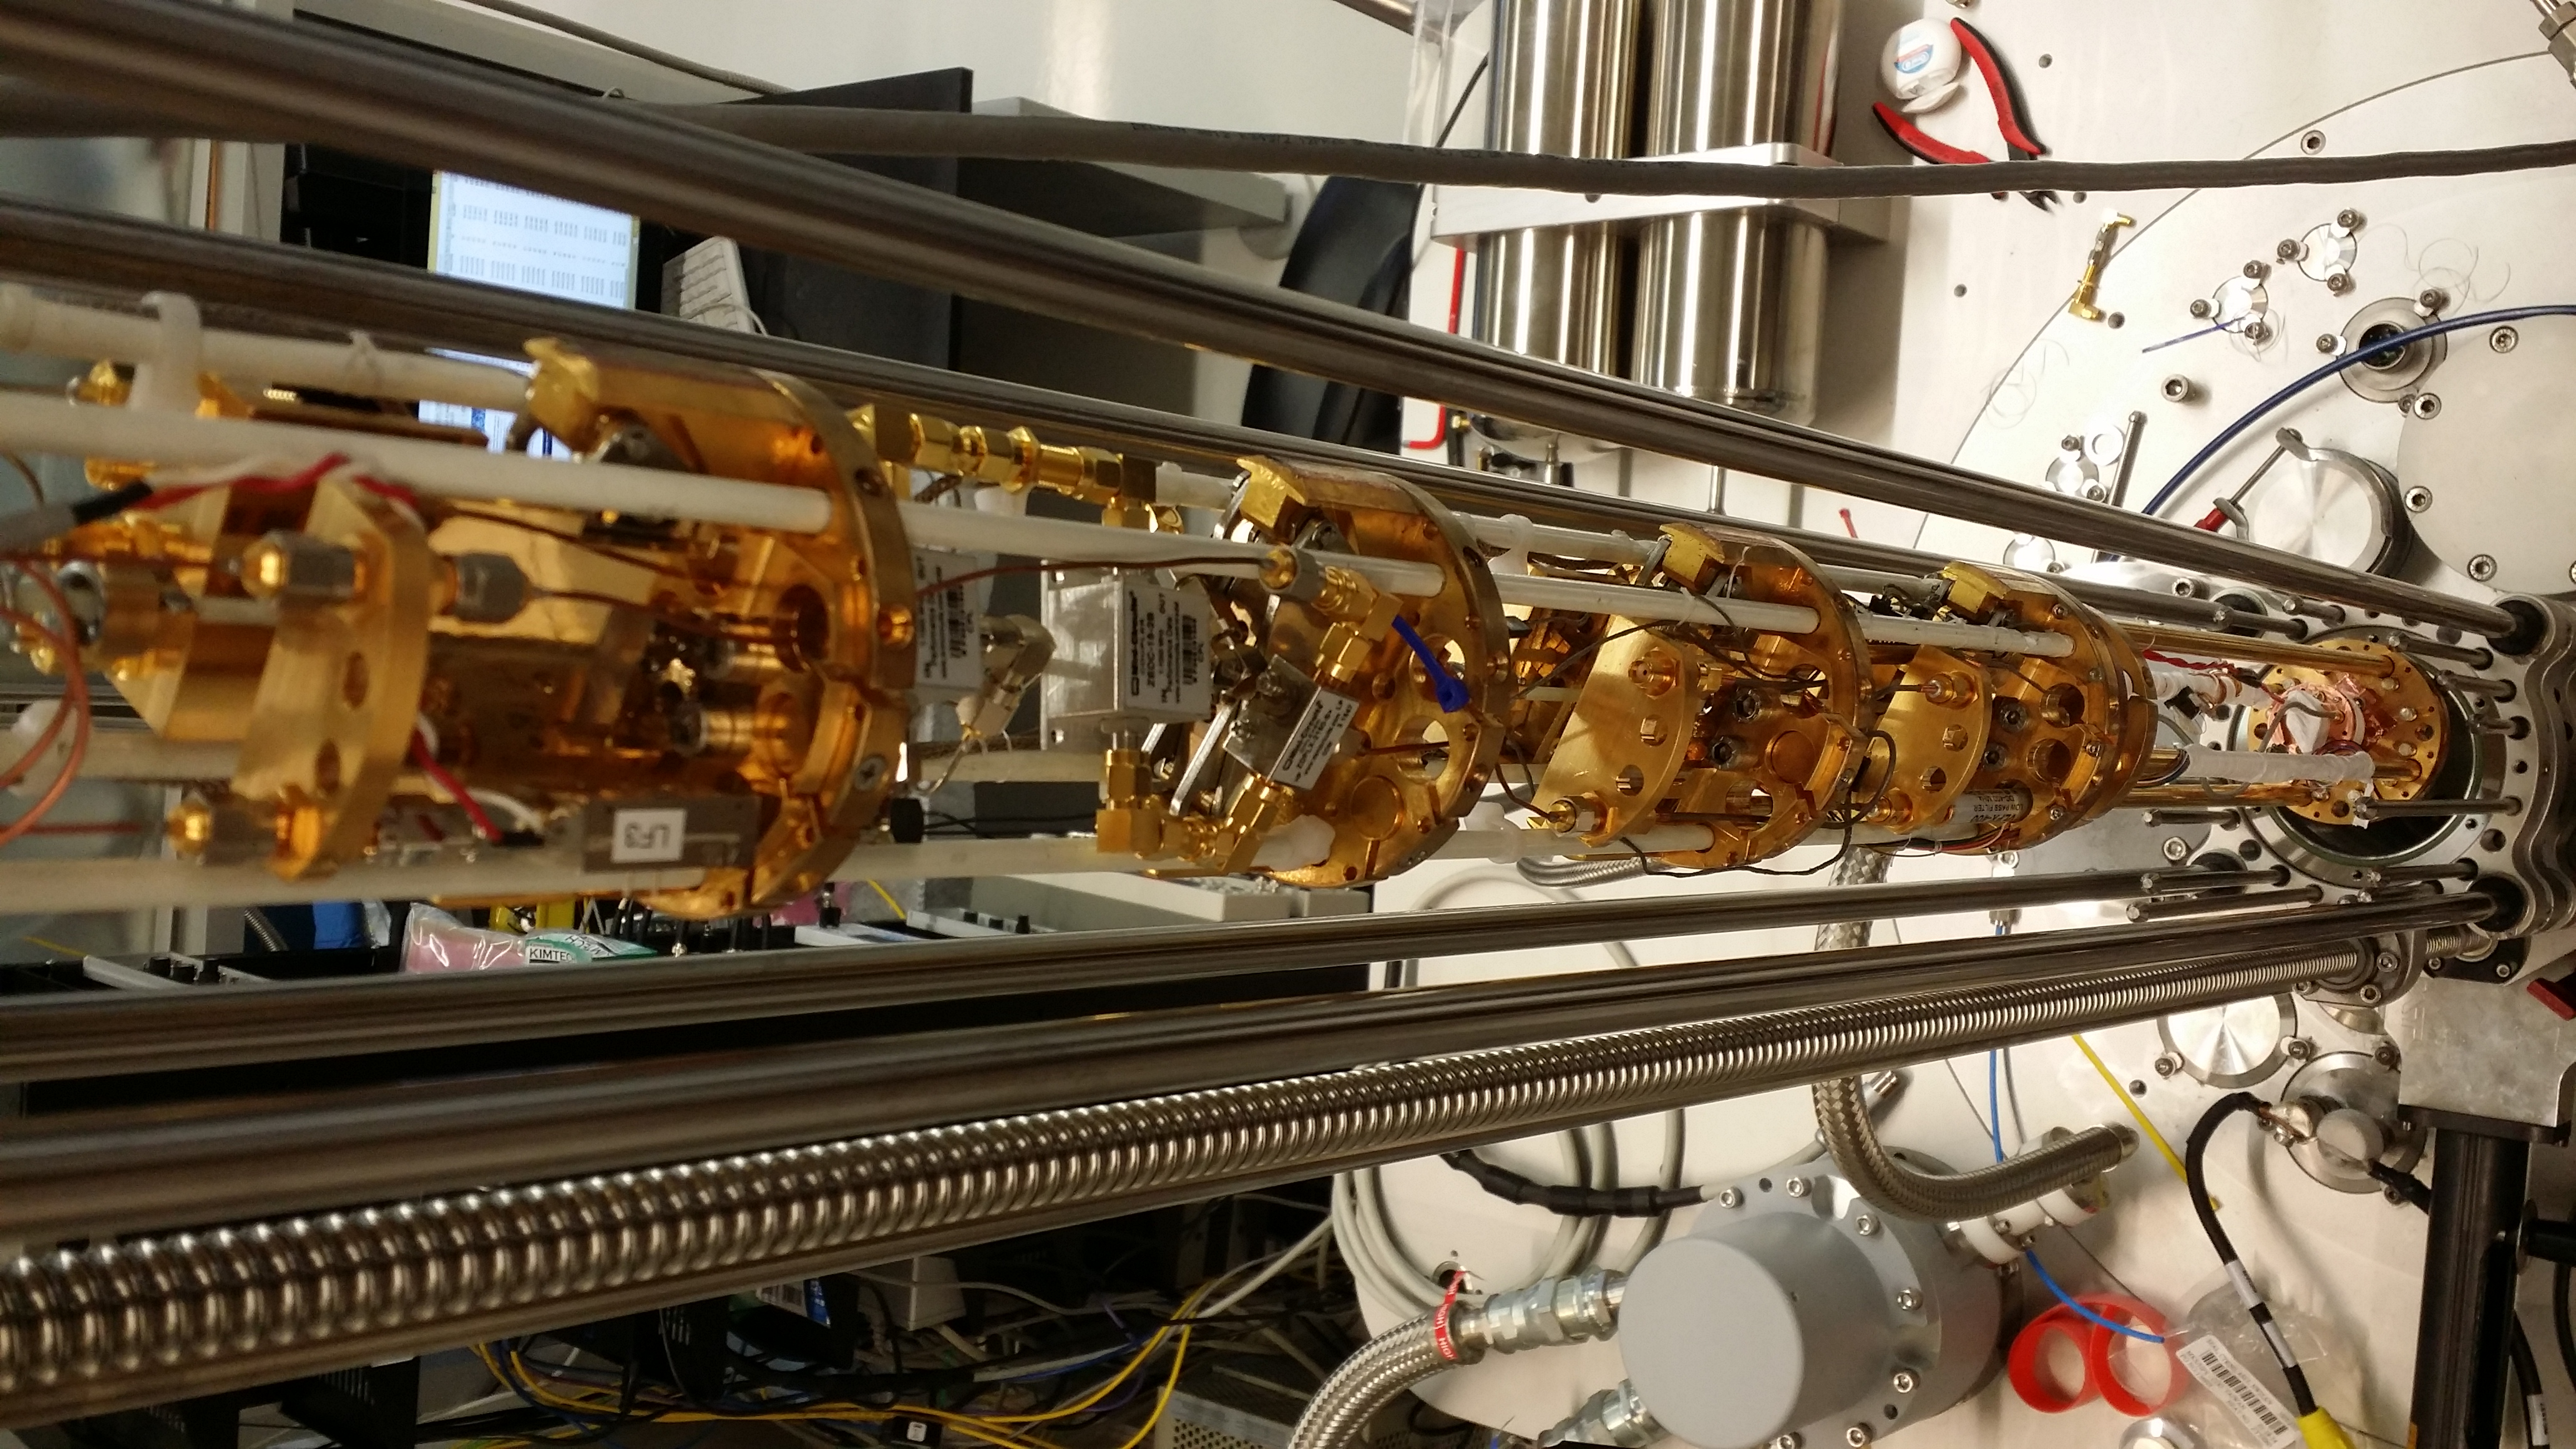
\includegraphics[angle=-90,width = 0.5\textwidth]{figures/appendix/cryostats/Leiden_probe.jpg}
\caption{An image of a microwave noise measurement circuit installed on the Leiden probe. A low noise amplifier is mounted to the $4~K$ plate and a bias-tee along with two directional couples are attached. This setup allows RF reflection and gain measurements of the sample and amplifier, respectively, as well as DC transport and RF noise measurements.}
\label{Fig:Appen:Leiden_probe}
\end{figure}

At the bottom of the probe (where the sample sits) is a plate with 16 SMP (smooth barrel) connectors pointing downward that fit into matching connectors installed in the main fridge body. When the probe is fully inserted, these connectors make an RF connection between the probe and the main body of the Leiden allowing experiments that require more complicated circuitry to use the ample space and cooling power of the main fridge. Fig. \ref{Fig:Appen:Leiden_clicking} shows an image of the underside of this ``clicking" mechanism where 16 SMA connectors can be used to probe the sample.

\begin{figure}
\centering
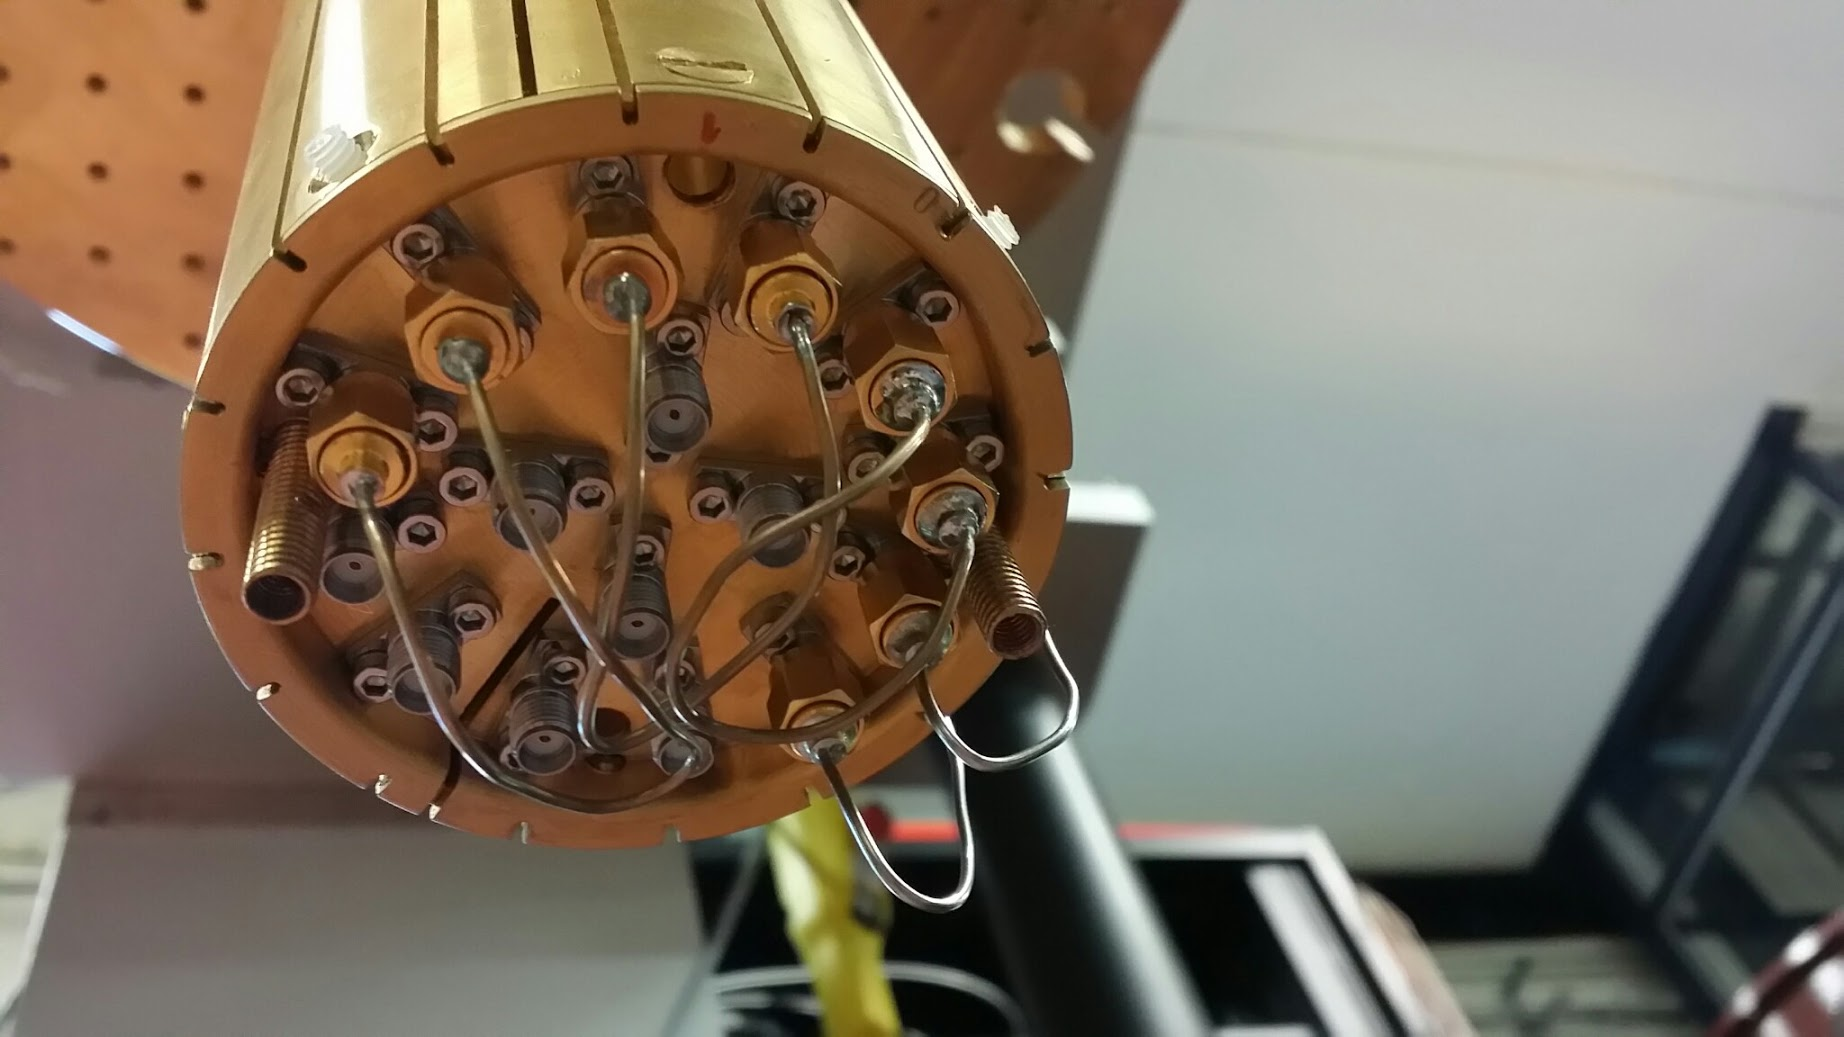
\includegraphics[width = 0.8\textwidth]{figures/appendix/cryostats/Leiden_clicking.jpg}
\caption{Image of the underside of the ''clicking" mechanism in the Leiden located in the main body of the fridge at the end of the tail that extends into the magnet bore. 16 SMA connectors are available and correspond to the 16 SMP connectors on the end of the probe. When the probe is fully inserted, these connectors form an RF connection between the probe and the main fridge body.}
\label{Fig:Appen:Leiden_clicking}
\end{figure}